\section{Results and Comparison to Simulation}
\label{chap:results}

\subsection{Corrected jet spectrum}
\label{sec:corrJetSpectrum}

\begin{figure}
    \centering
    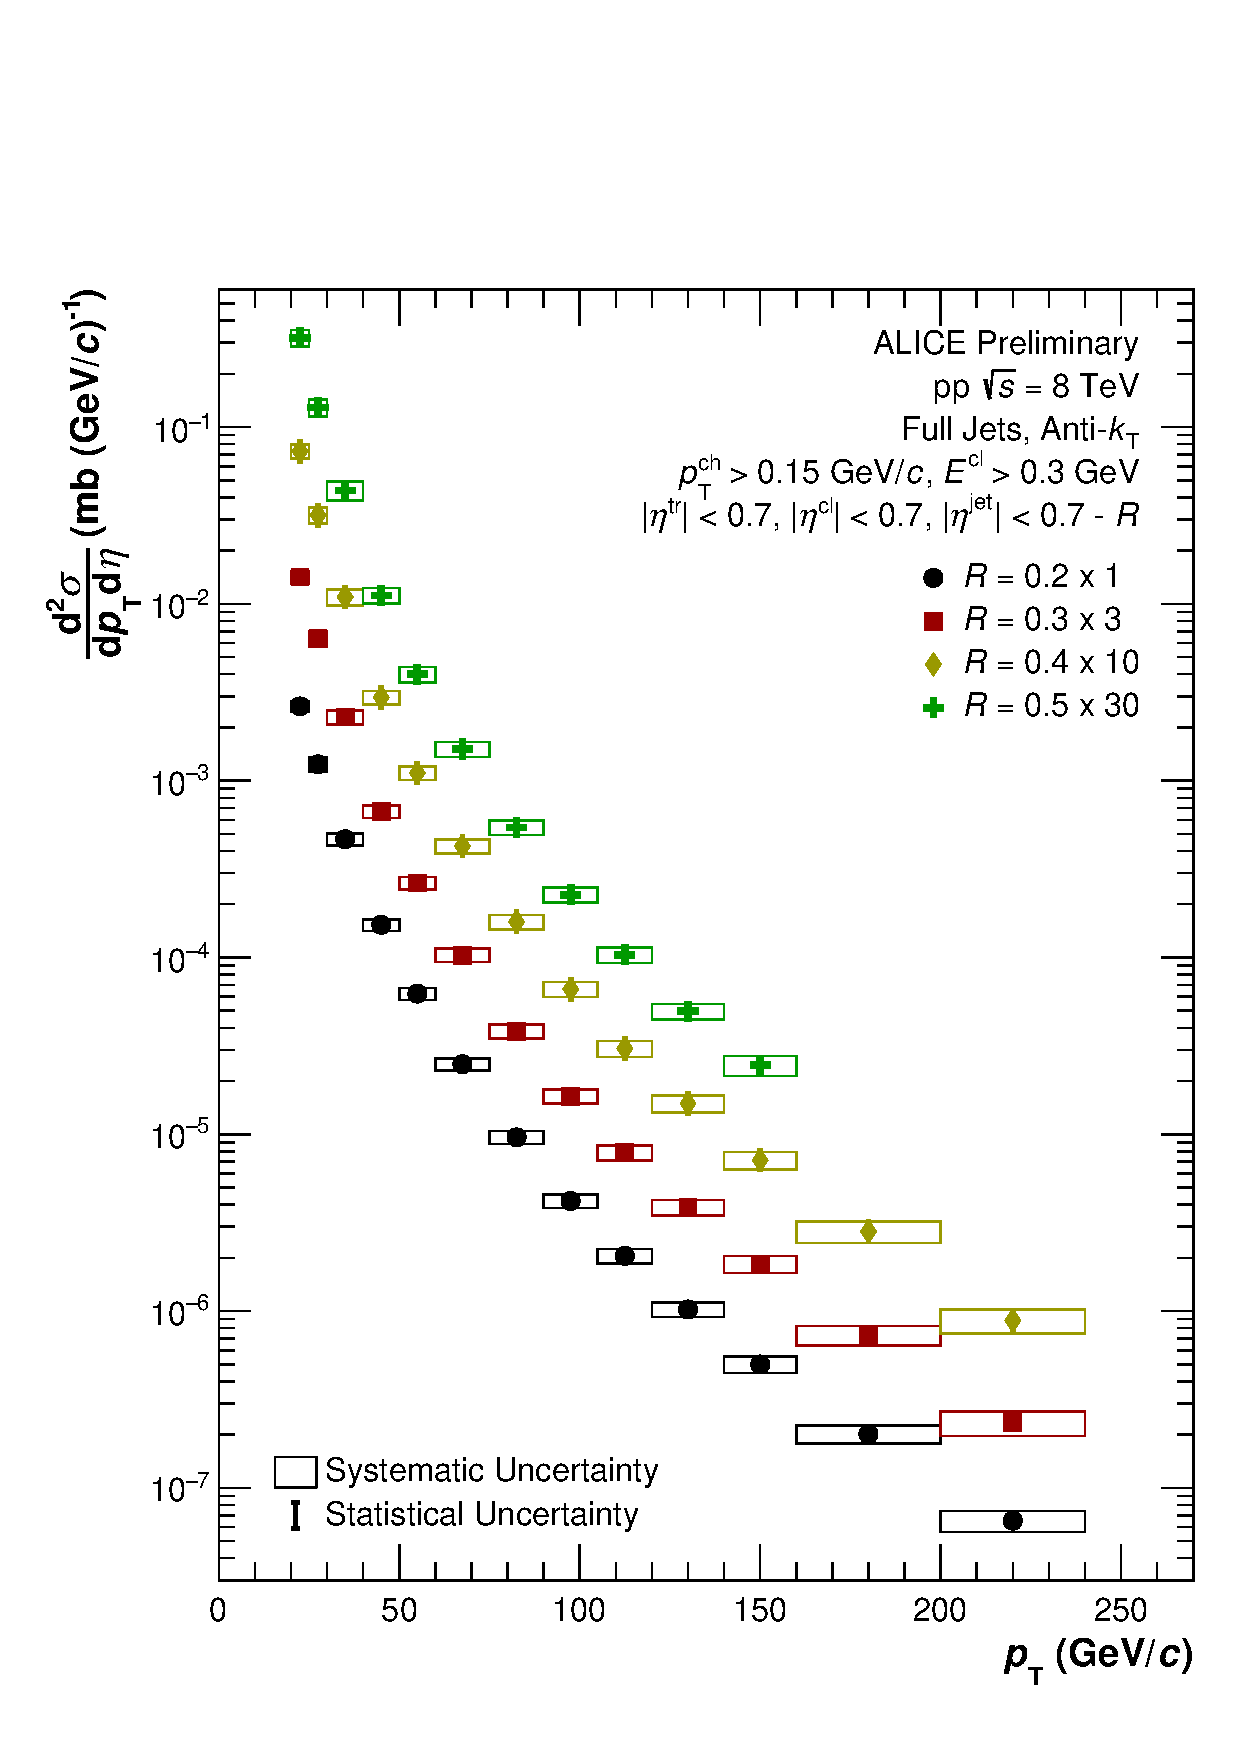
\includegraphics[width=15cm]{figures/FinalResults/Bayes_reg6.pdf}
    \caption{Jet spectra in \pp for various jet radii after corrections, unfolding, and addition of systematic errors. Scaled for visual clarity.}
    \label{fig:finalSpectra}
\end{figure}

\begin{figure}
    \centering
    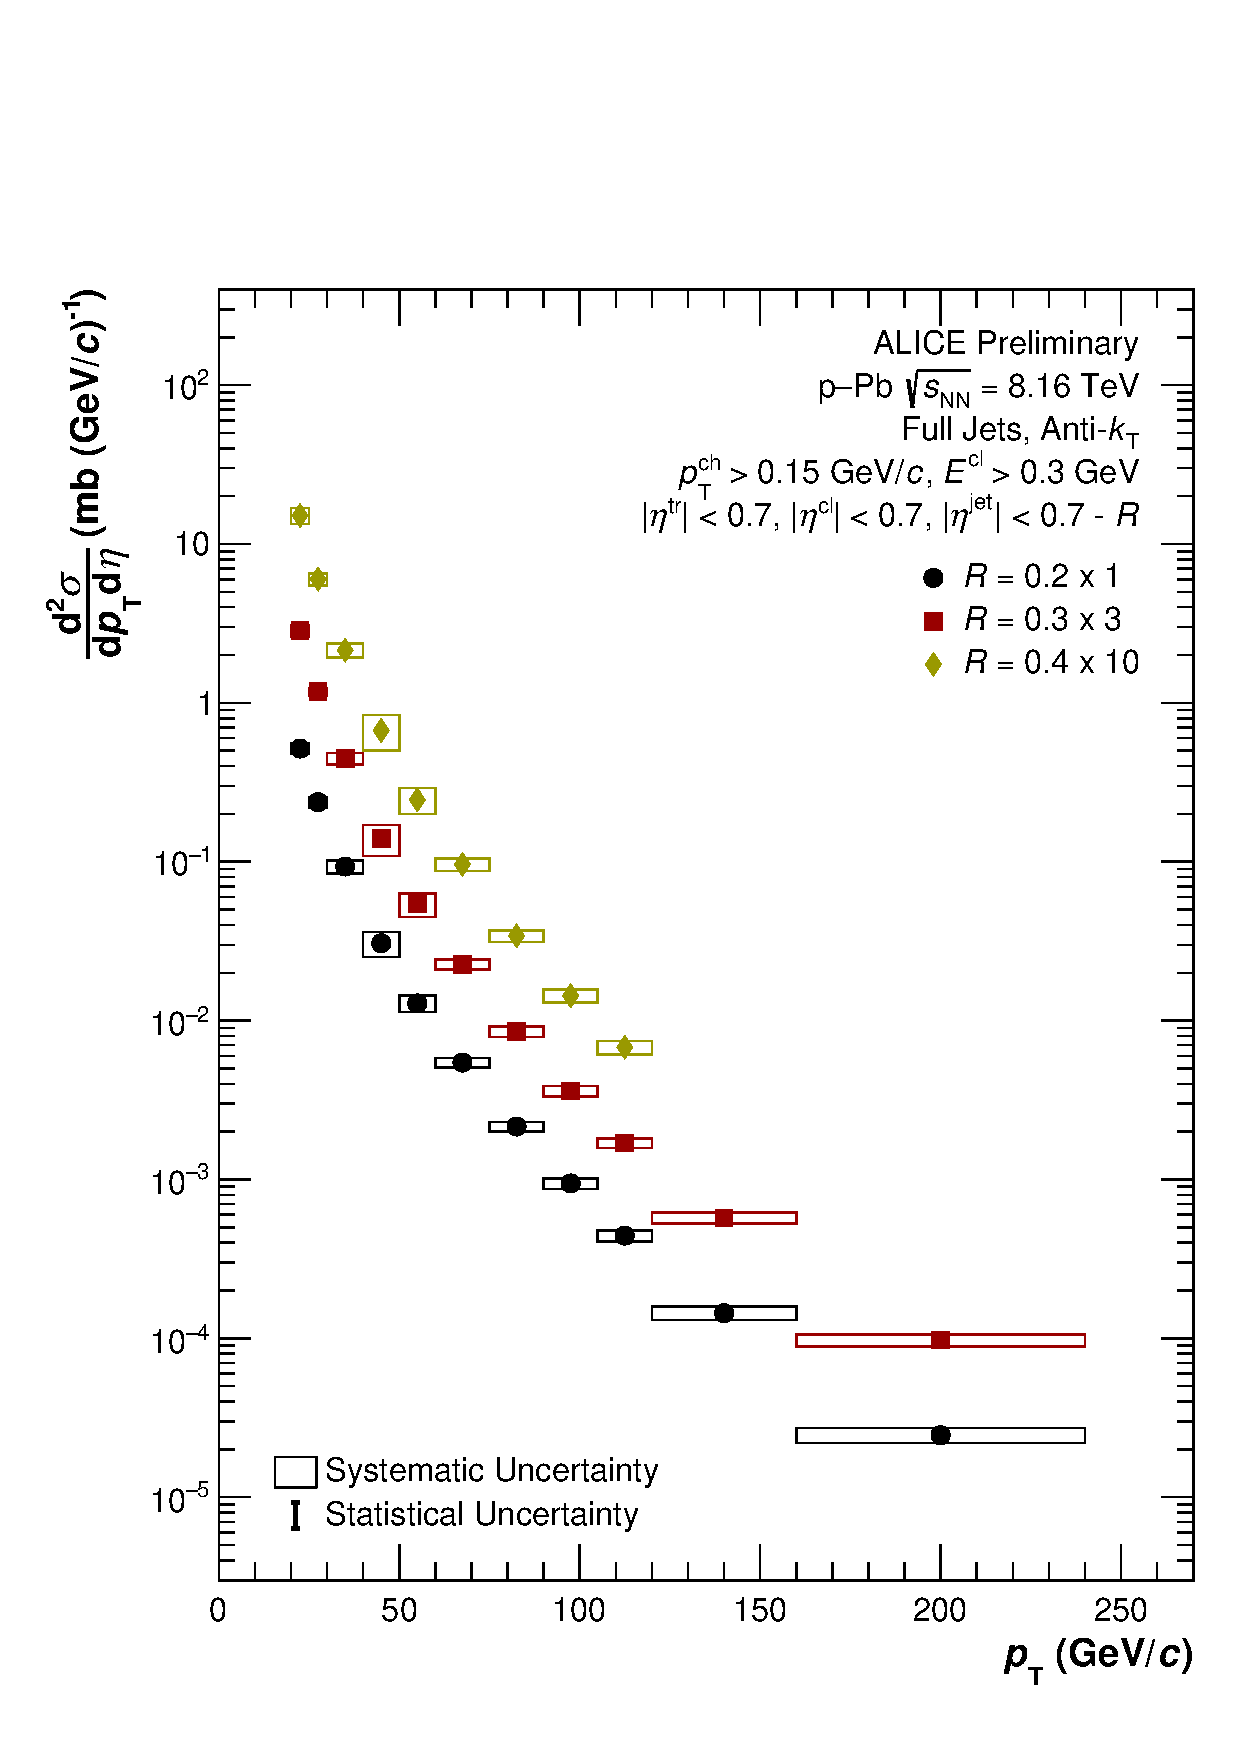
\includegraphics[width=15cm]{figures/pPbFigures/FinalResults/Bayes_reg6.pdf}
    \caption{Jet spectra in \pPb for various jet radii after corrections, unfolding, and addition of systematic errors. Scaled for visual clarity.}
    \label{fig:finalSpectrapPb}
\end{figure}

\begin{figure}
    \centering
    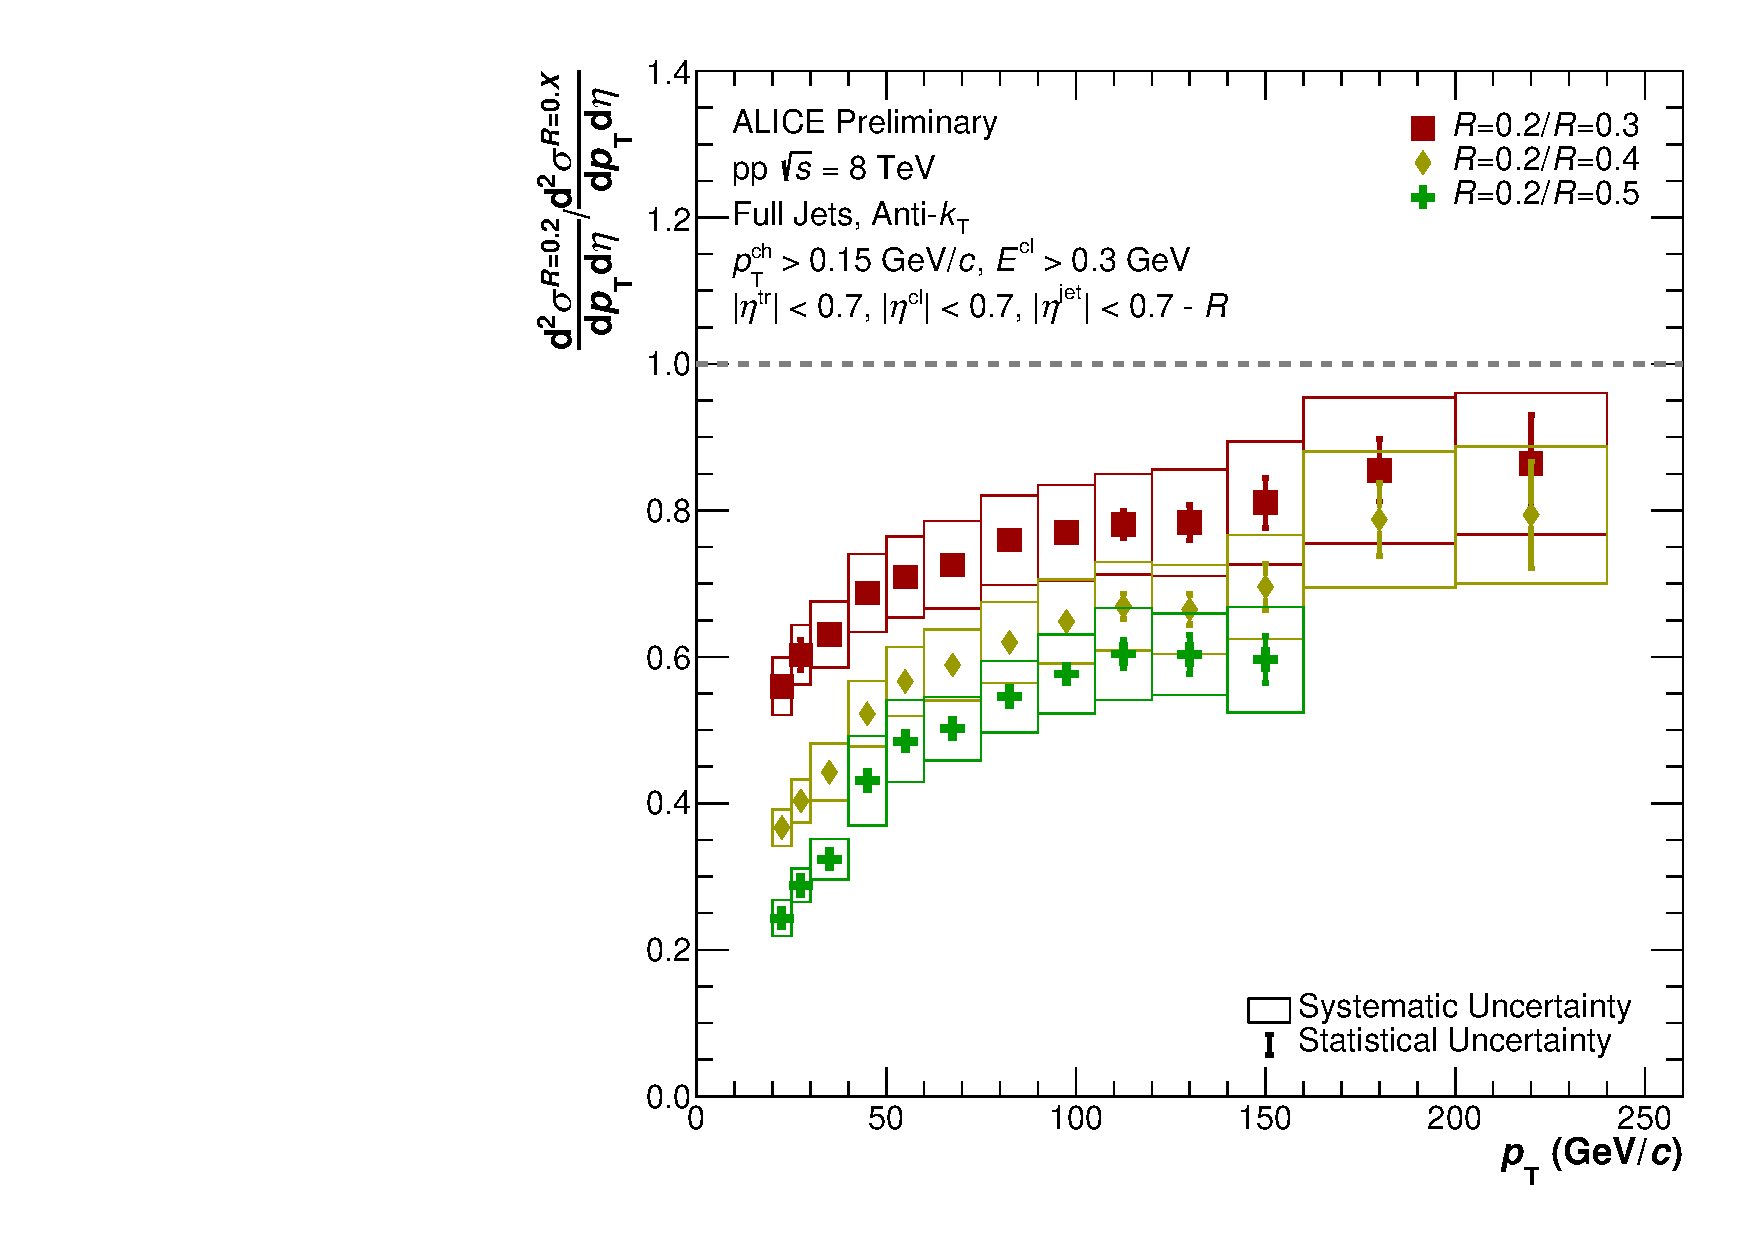
\includegraphics[width=15cm]{figures/FinalResults/Bayes_reg6_Ratio.pdf}
    \caption{Jet spectra in \pp for various jet radii compared to R = 0.2 after corrections, unfolding, and addition of systematic errors.}
    \label{fig:finalSpectraRatios}
\end{figure}

\begin{figure}
    \centering
    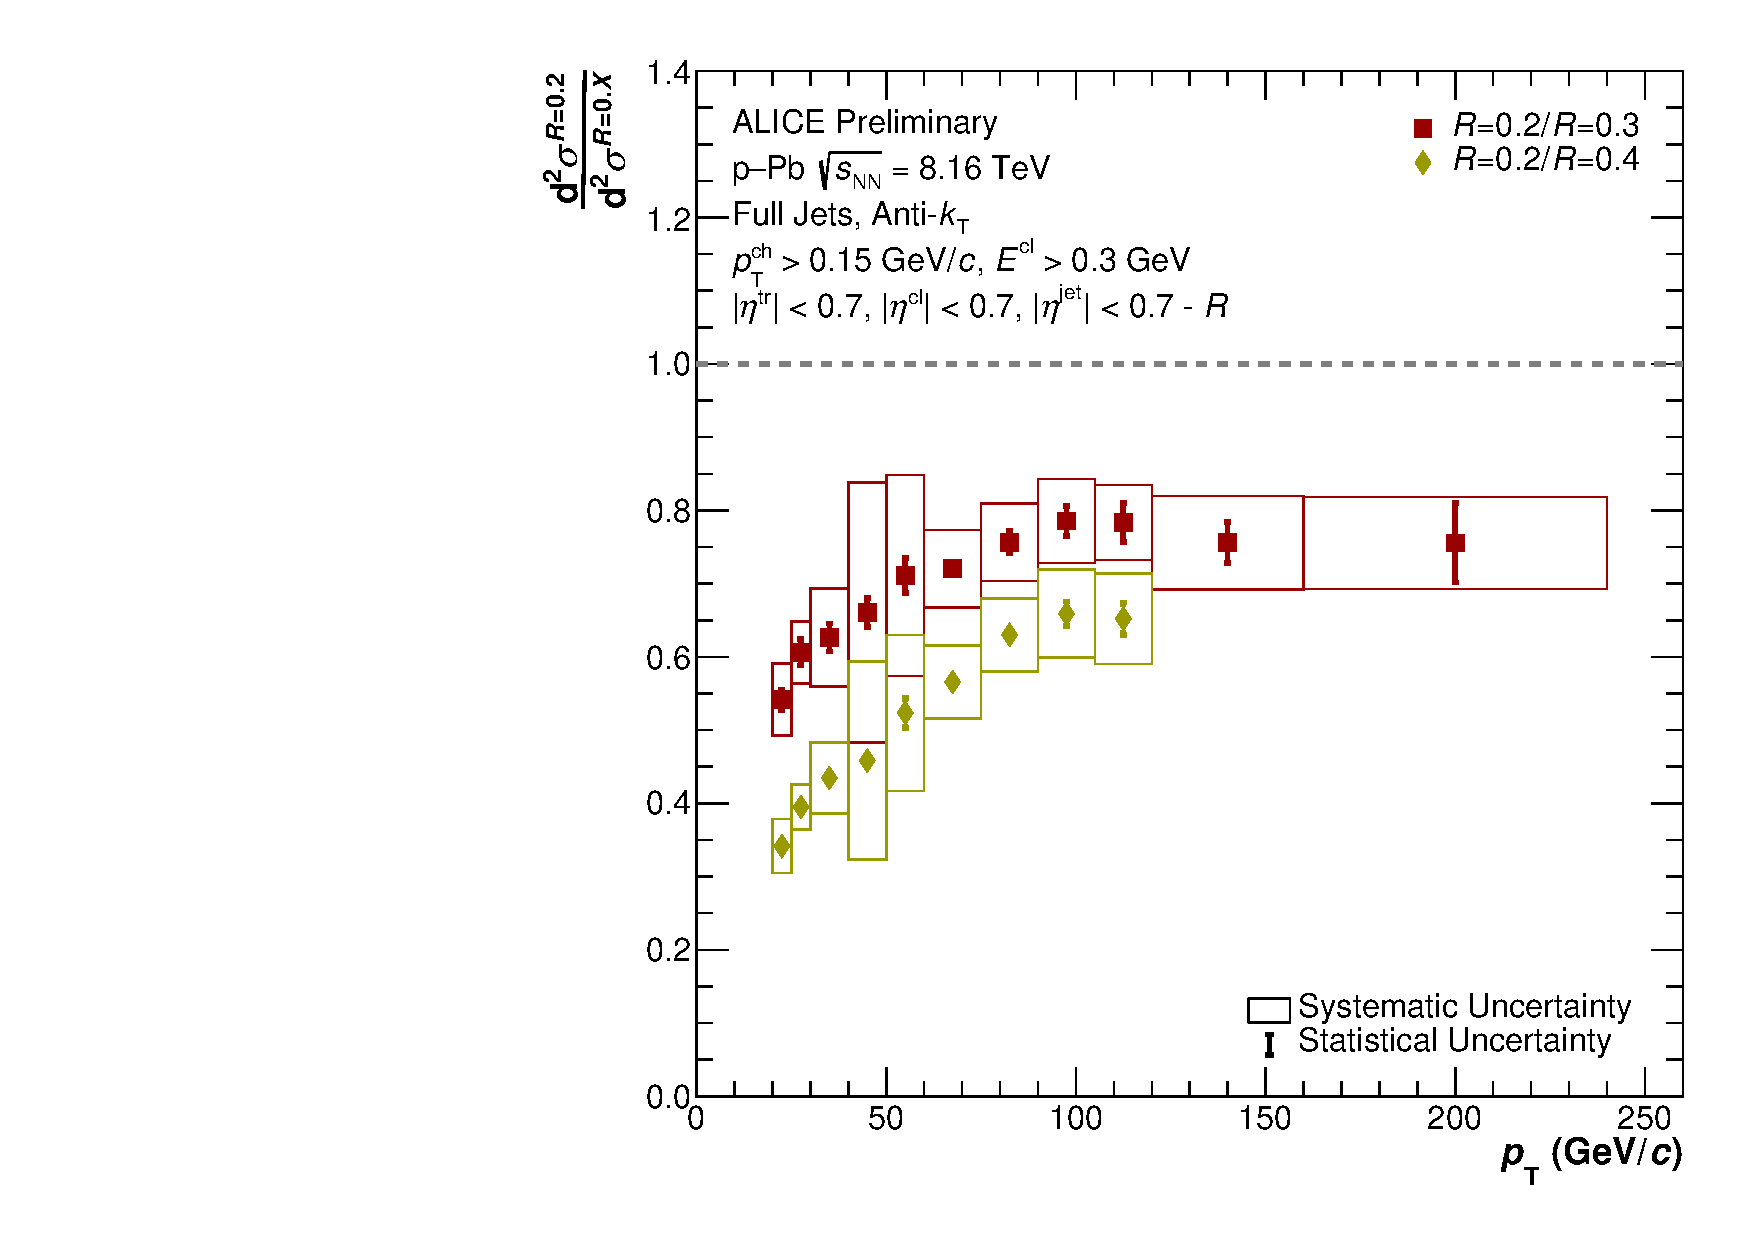
\includegraphics[width=15cm]{figures/pPbFigures/FinalResults/Bayes_reg6_Ratio.pdf}
    \caption{Jet spectra in \pPb for various jet radii compared to R = 0.2 after corrections, unfolding, and addition of systematic errors.}
    \label{fig:finalSpectraRatiospPb}
\end{figure}

Fig. \ref{fig:finalSpectra} and \ref{fig:finalSpectrapPb} show the comparison of the jet \pT spectra for the different jet radii, while fig. \ref{fig:finalSpectraRatios} and \ref{fig:finalSpectraRatiospPb} show the ratio of R = 0.2 and the remaining radii. Three plotting variations of the final spectra can be found in figures \ref{fig:finalSpectraLogX}, \ref{fig:finalSpectraUnscaled}, and \ref{fig:finalSpectraUnscaledLogX}.
The measurements are shown in the selected \pT regions.

\begin{figure}
    \centering
    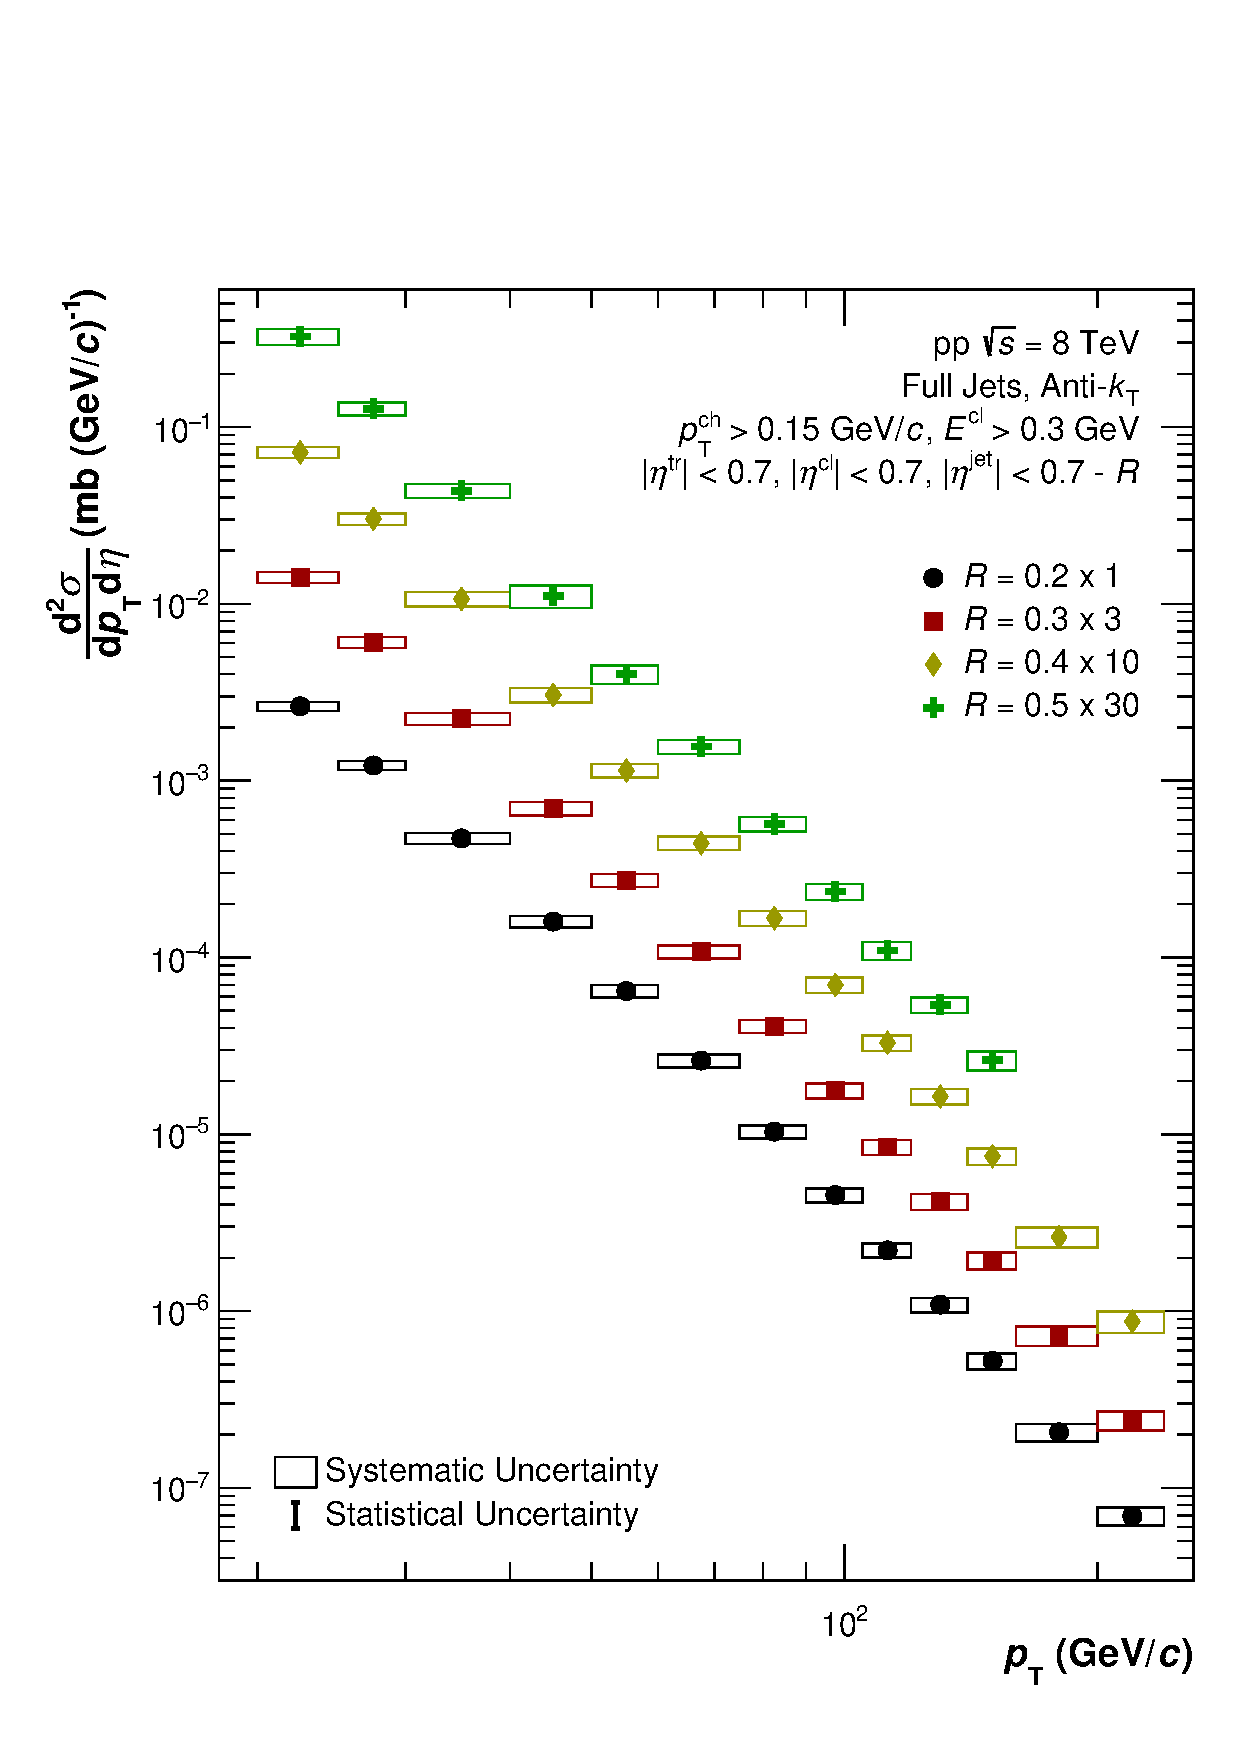
\includegraphics[width=7.5cm]{figures/FinalResults/Bayes_reg6_logx.pdf}
    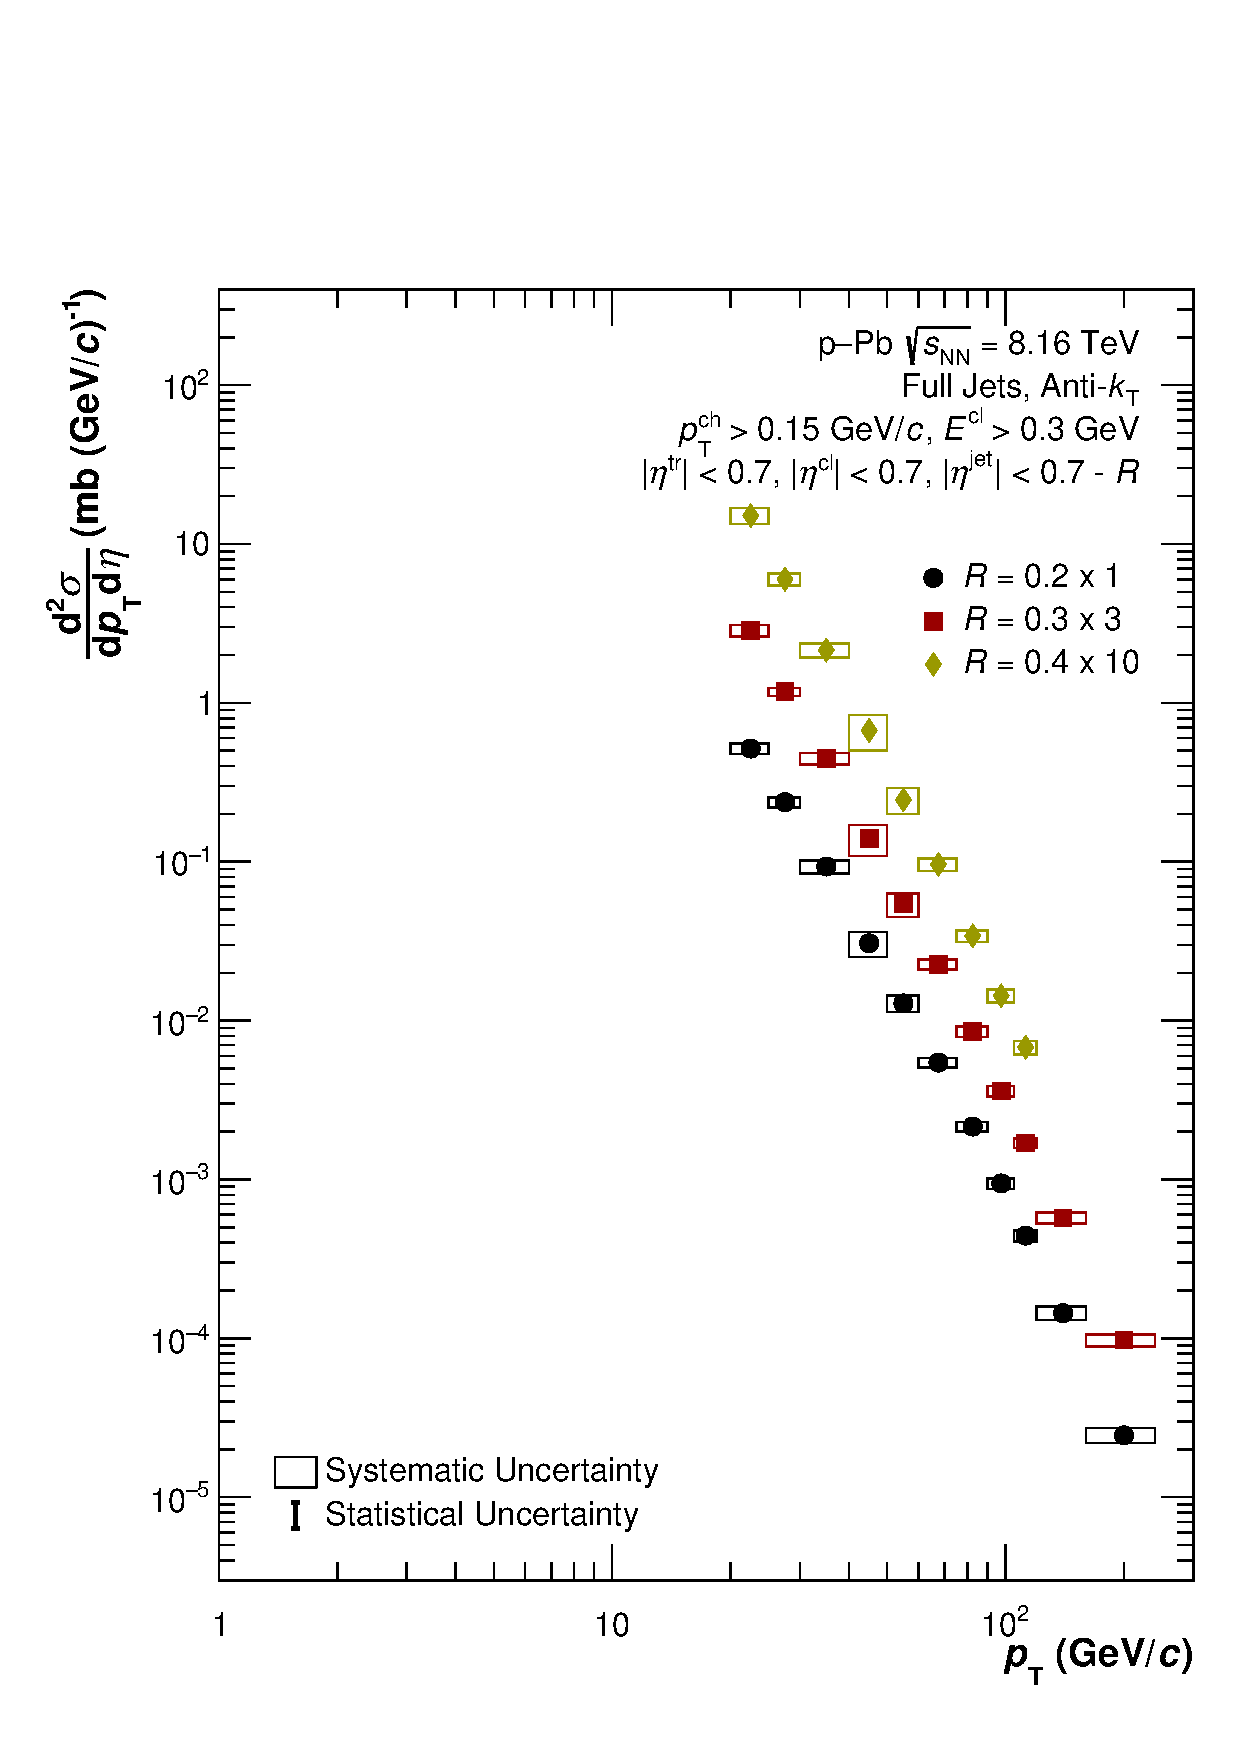
\includegraphics[width=7.5cm]{figures/pPbFigures/FinalResults/Bayes_reg6_logx.pdf}
    \caption{Jet spectra with a logarithmic x-axis for various jet radii after corrections, unfolding, and addition of systematic errors. Scaled for visual clarity. \pp (left) and \pPb (right).}
    \label{fig:finalSpectraLogX}
\end{figure}

\begin{figure}
    \centering
    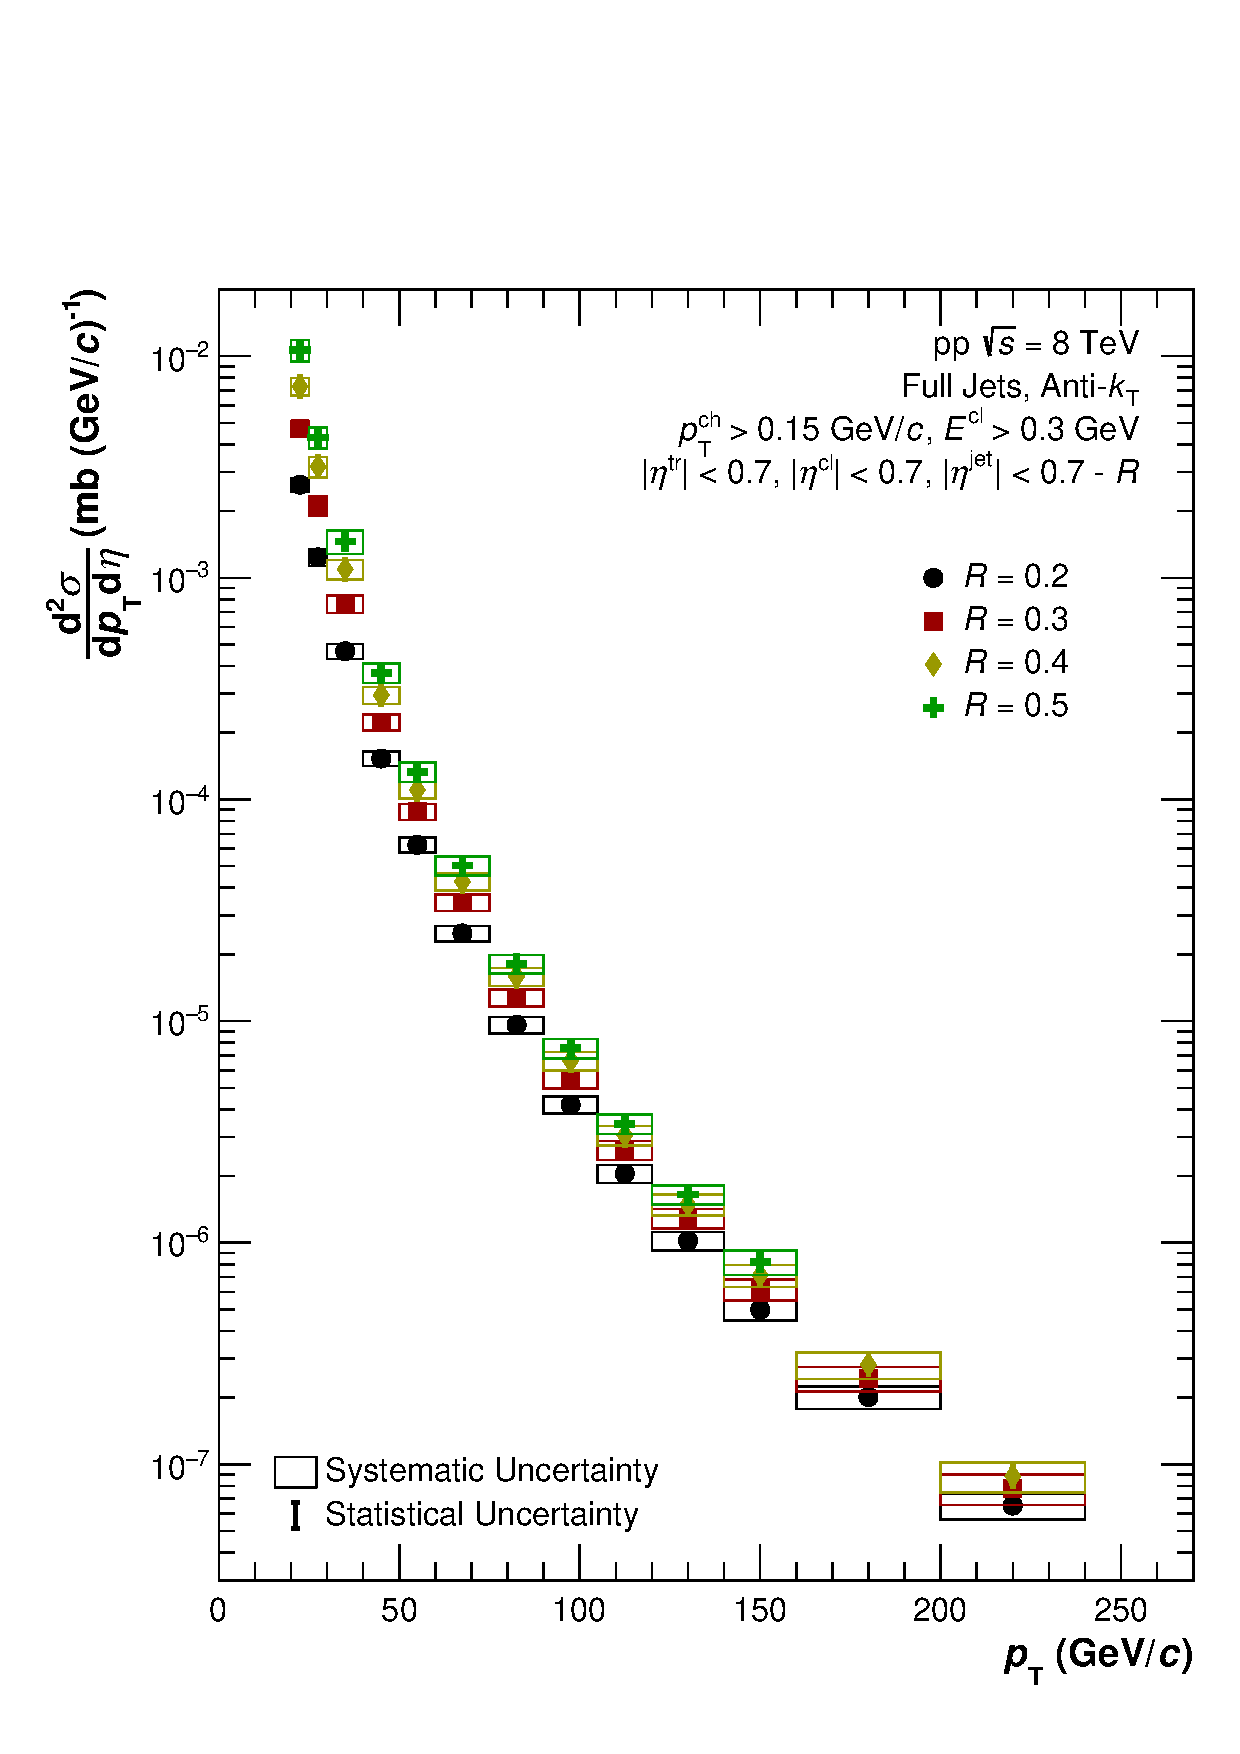
\includegraphics[width=7.5cm]{figures/FinalResults/Bayes_reg6_unscaled.pdf}
    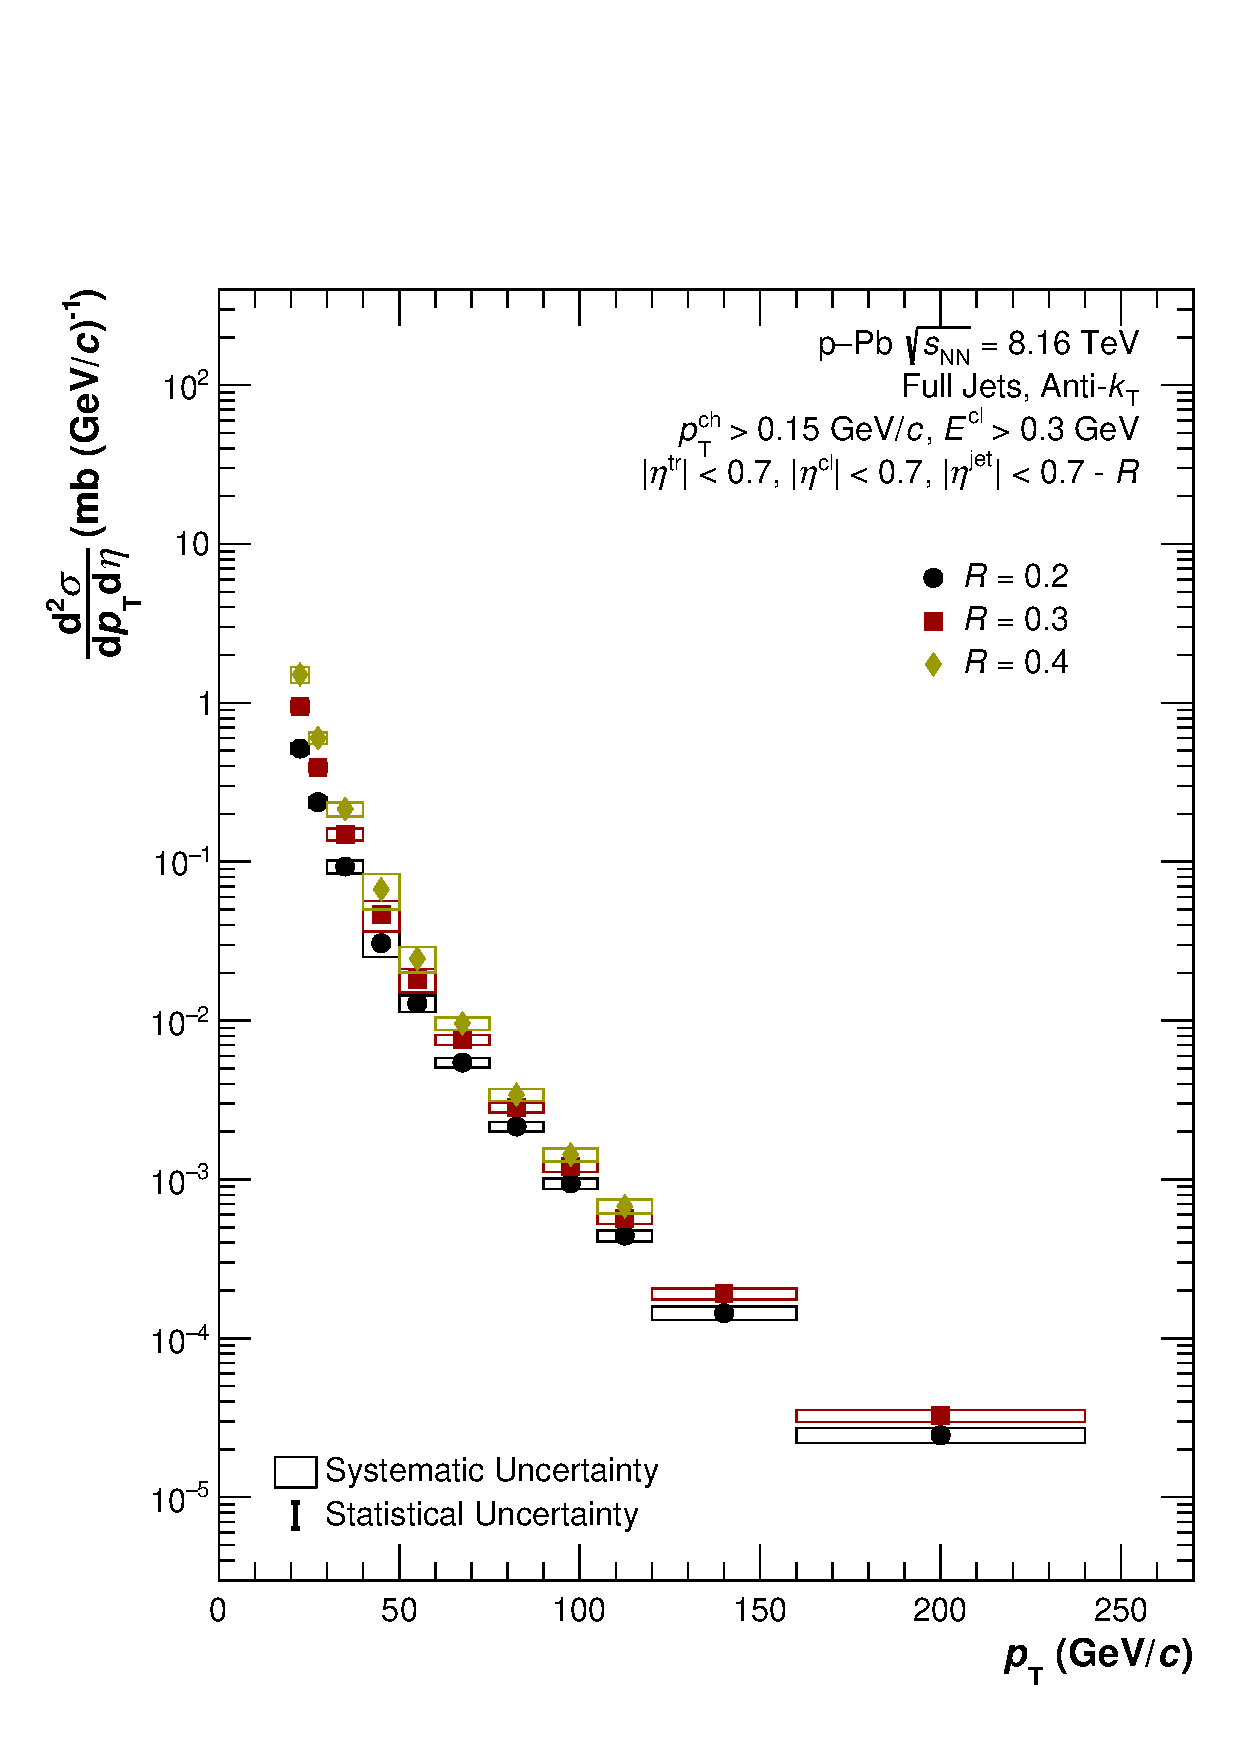
\includegraphics[width=7.5cm]{figures/pPbFigures/FinalResults/Bayes_reg6_unscaled.pdf}
    \caption{Jet spectra for various jet radii after corrections, unfolding, and addition of systematic errors. Unscaled. \pp (left) and \pPb (right).}
    \label{fig:finalSpectraUnscaled}
\end{figure}

\begin{figure}
    \centering
    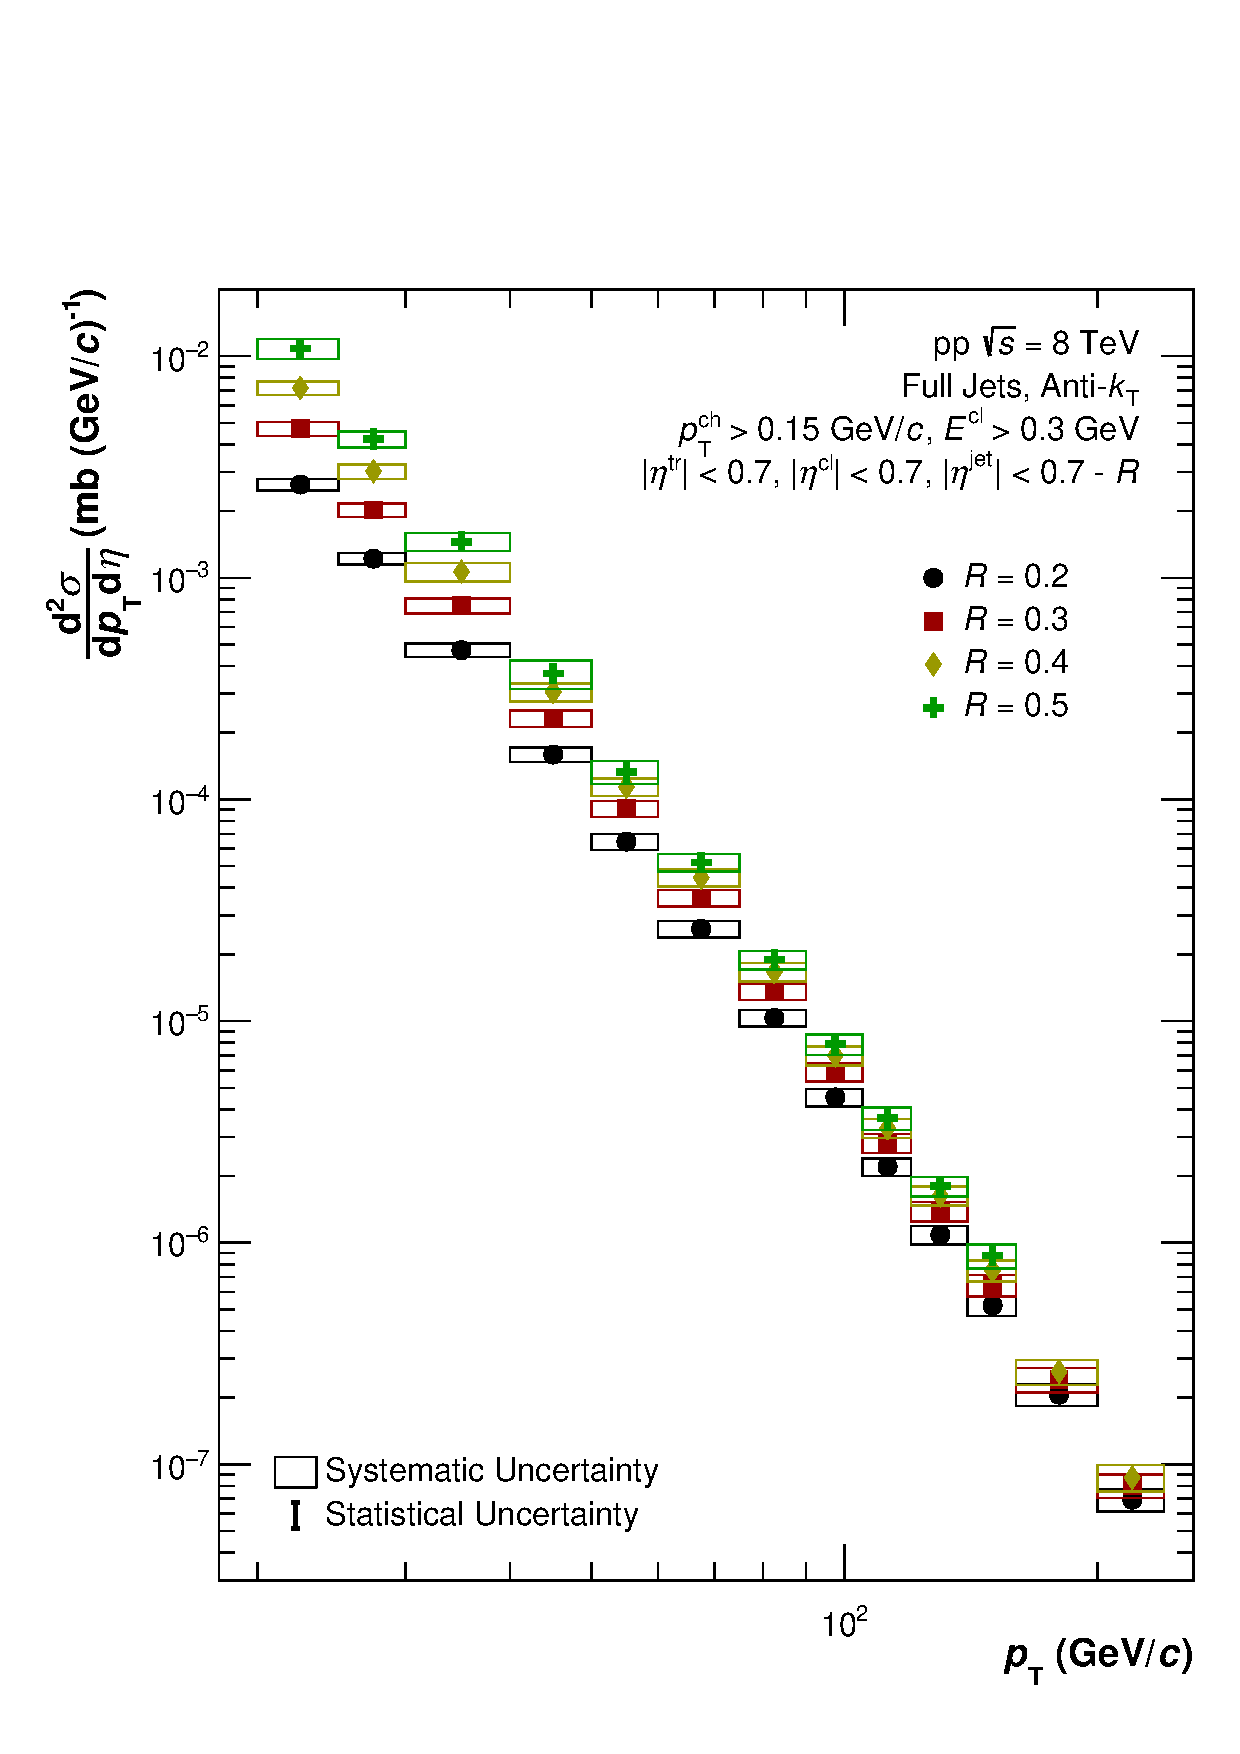
\includegraphics[width=7.5cm]{figures/FinalResults/Bayes_reg6_logx_unscaled.pdf}
    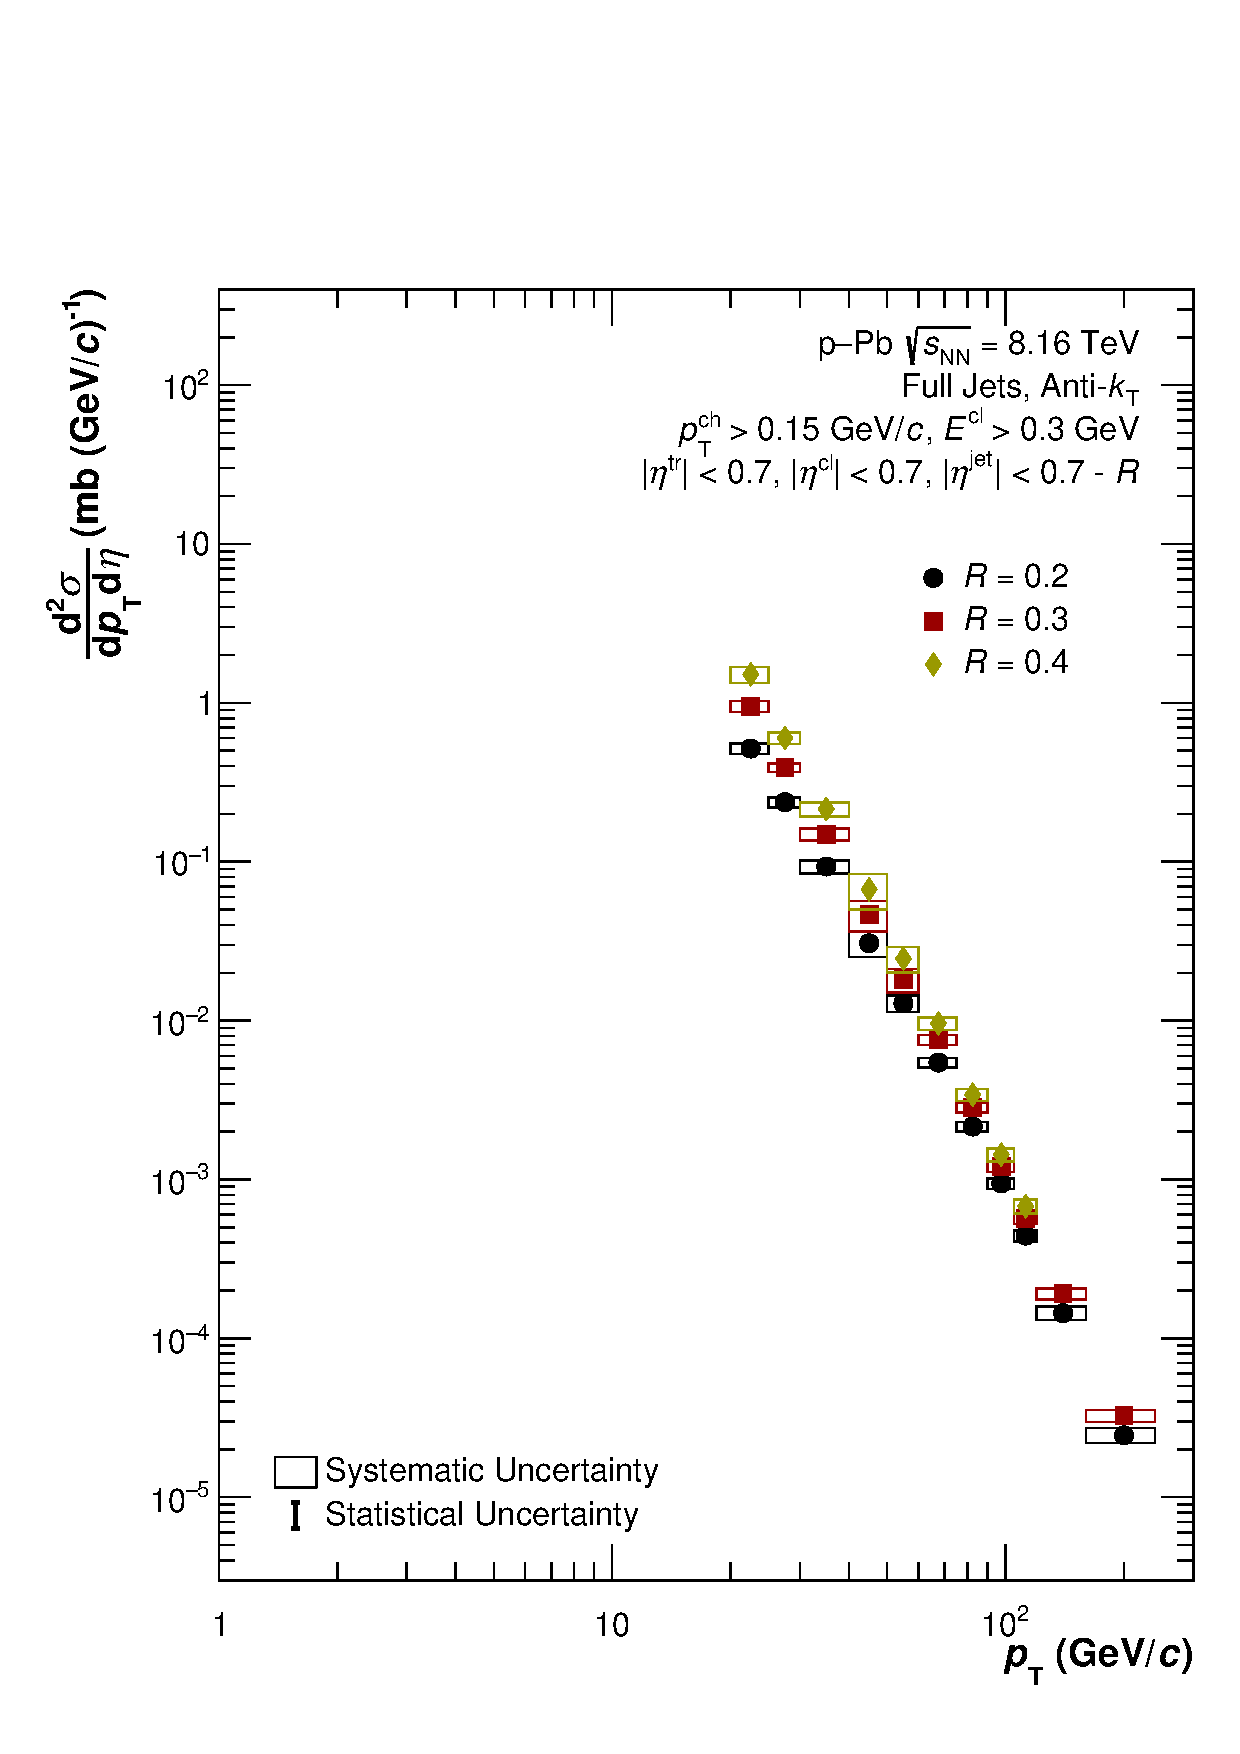
\includegraphics[width=7.5cm]{figures/pPbFigures/FinalResults/Bayes_reg6_logx_unscaled.pdf}
    \caption{Jet spectra with a logarithmic x-axis for various jet radii after corrections, unfolding, and addition of systematic errors. Unscaled. \pp (left) and \pPb (right).}
    \label{fig:finalSpectraUnscaledLogX}
\end{figure}

\subsection{Nuclear modification factor}
\label{sec:resultsRpA}

The nuclear modification factor is found by taking the ratio of the jet cross-section in \pPb to that in \pp scaled by 208. Alternate, equivalent methods for calculating the \RpPb are 

\begin{equation}
    \text{\RpPb}(\text{\pT}) = \frac{1}{208} \frac{ d\sigma^{\text{pPb}}/d\text{\pT} }{ d\sigma^{\text{\pp}}/d\text{\pT} } = \frac{1}{T_\text{pPb}} \frac{ dN^{\text{pPb}}/d\text{\pT} }{ d\sigma^{\text{\pp}}/d\text{\pT} } = \frac{1}{\langle N_\text{coll}\rangle} \frac{ dN^{\text{pPb}}/d\text{\pT} }{ dN^{\text{\pp}}/d\text{\pT} }
    \label{eq:RpPb_equation}
\end{equation}

\noindent
where $\sigma$ are the cross-sections for \pp and \pPb, $N$ are the yields, $T_{\text{pPb}}$ is the nuclear overlap function, and $\langle N_\text{coll}\rangle$ is the average number of binary nucleon-nucleon collisions. The latter two values are extracted from Glauber models. Because the center of mass energy of \pPb collisions for this measurement is 8.16 TeV while the center of mass energy for \pp collisions is 8 TeV, the \pp spectrum must be scaled from 8 TeV to 8.16 TeV to be consistent with the \pPb spectrum. This is performed by taking the ratio of generated PYTHIA jets in 8.16 and 8 TeV and applying this as a momentum-dependent scaling factor to the \pp spectrum, effectively giving the \pp spectrum at 8.16 TeV. By using PYTHIA to scale the spectrum, a model dependence is introduced into the measurement, although small. The small rapidity shift introduced in \pPb collisions is not accounted for in the generated PYTHIA events. The scaling factor is on the order of approximately 3\%, which is comparable to the level of the statistical uncertainty on the spectrum and far below the systematic uncertainty. For $R$ = 0.2, the scaling factor is shown in Figure~\ref{fig:PythiaScaleFactor}. The scale factors for the remaining radii are nearly identical and can be found in Appendix~\ref{sec:appendixScaleFactors}.

\begin{figure}[hbt!]
    \centering
    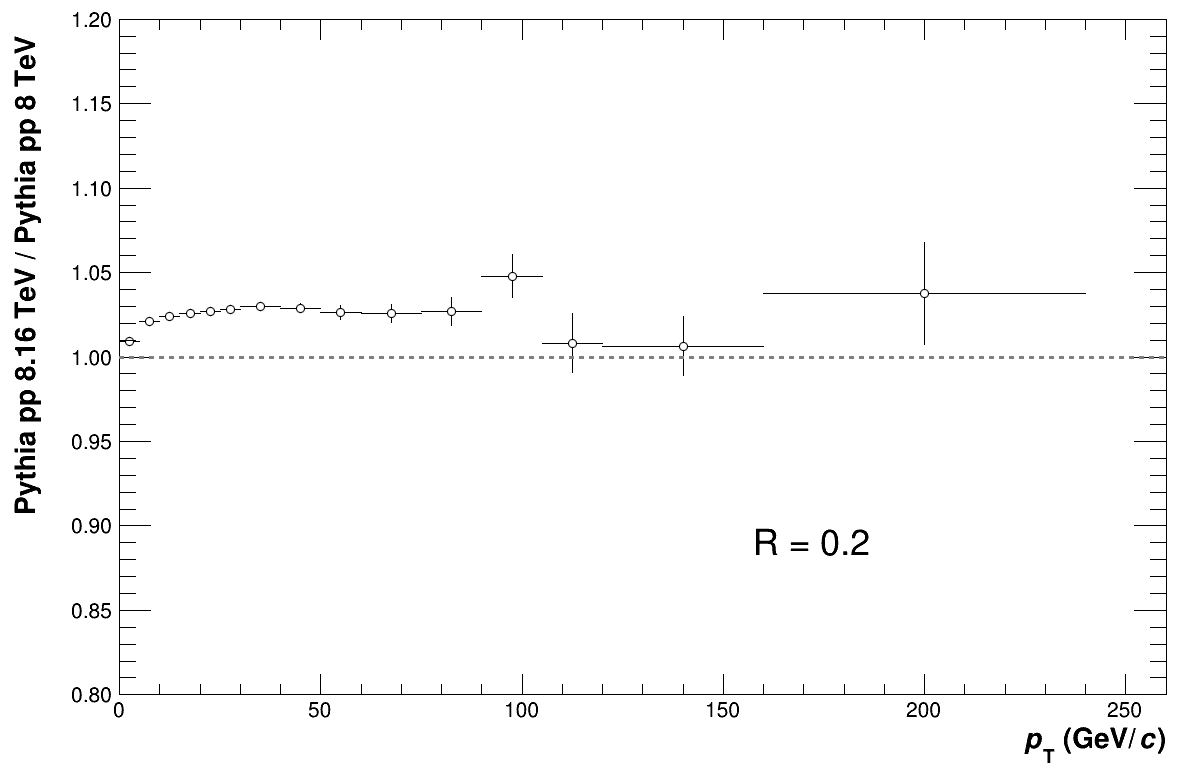
\includegraphics[width=\textwidth]{figures/ScaleFactorPythia/PythiaRatio_R02.png}
    \caption{Ratio of generated \pp PYTHIA events at 8.16 TeV to 8 TeV for $R$ = 0.2 jets.}
    \label{fig:PythiaScaleFactor}
\end{figure}

The nuclear modification factor for R = 0.2 to 0.4 can be found in Figure~\ref{fig:finalRpPb}. For R = 0.4 and R = 0.3, the \RpPb is consistent with unity within uncertainties. With R = 0.2 jets, the ratio begins to deviate from 1 at high-\pT, suggesting a possible presence of jet modification for jets with small resolution parameters.

\begin{figure}[hbt!]
    \centering
    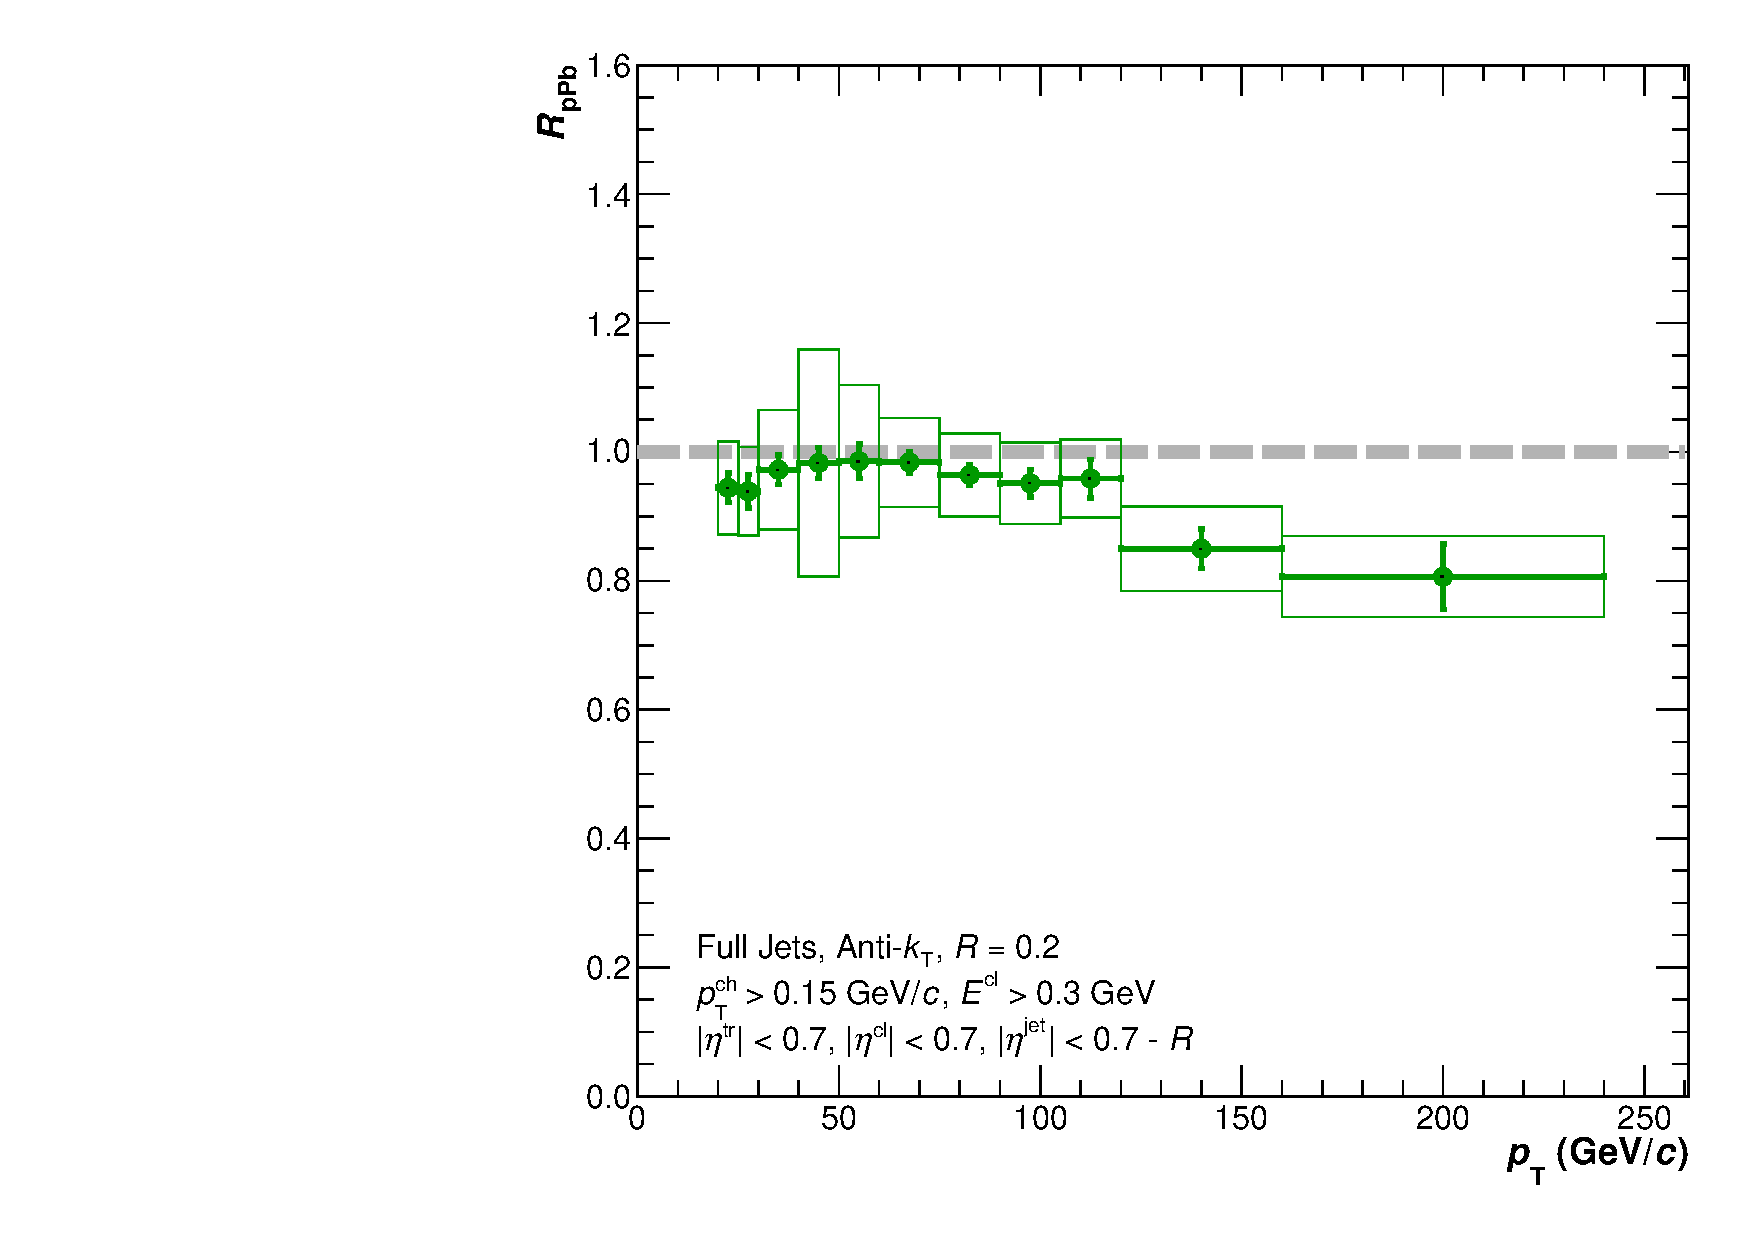
\includegraphics[width=0.49\textwidth]{figures/pPbFigures/RpPb/ptscheme/RpPb_R02.pdf}
    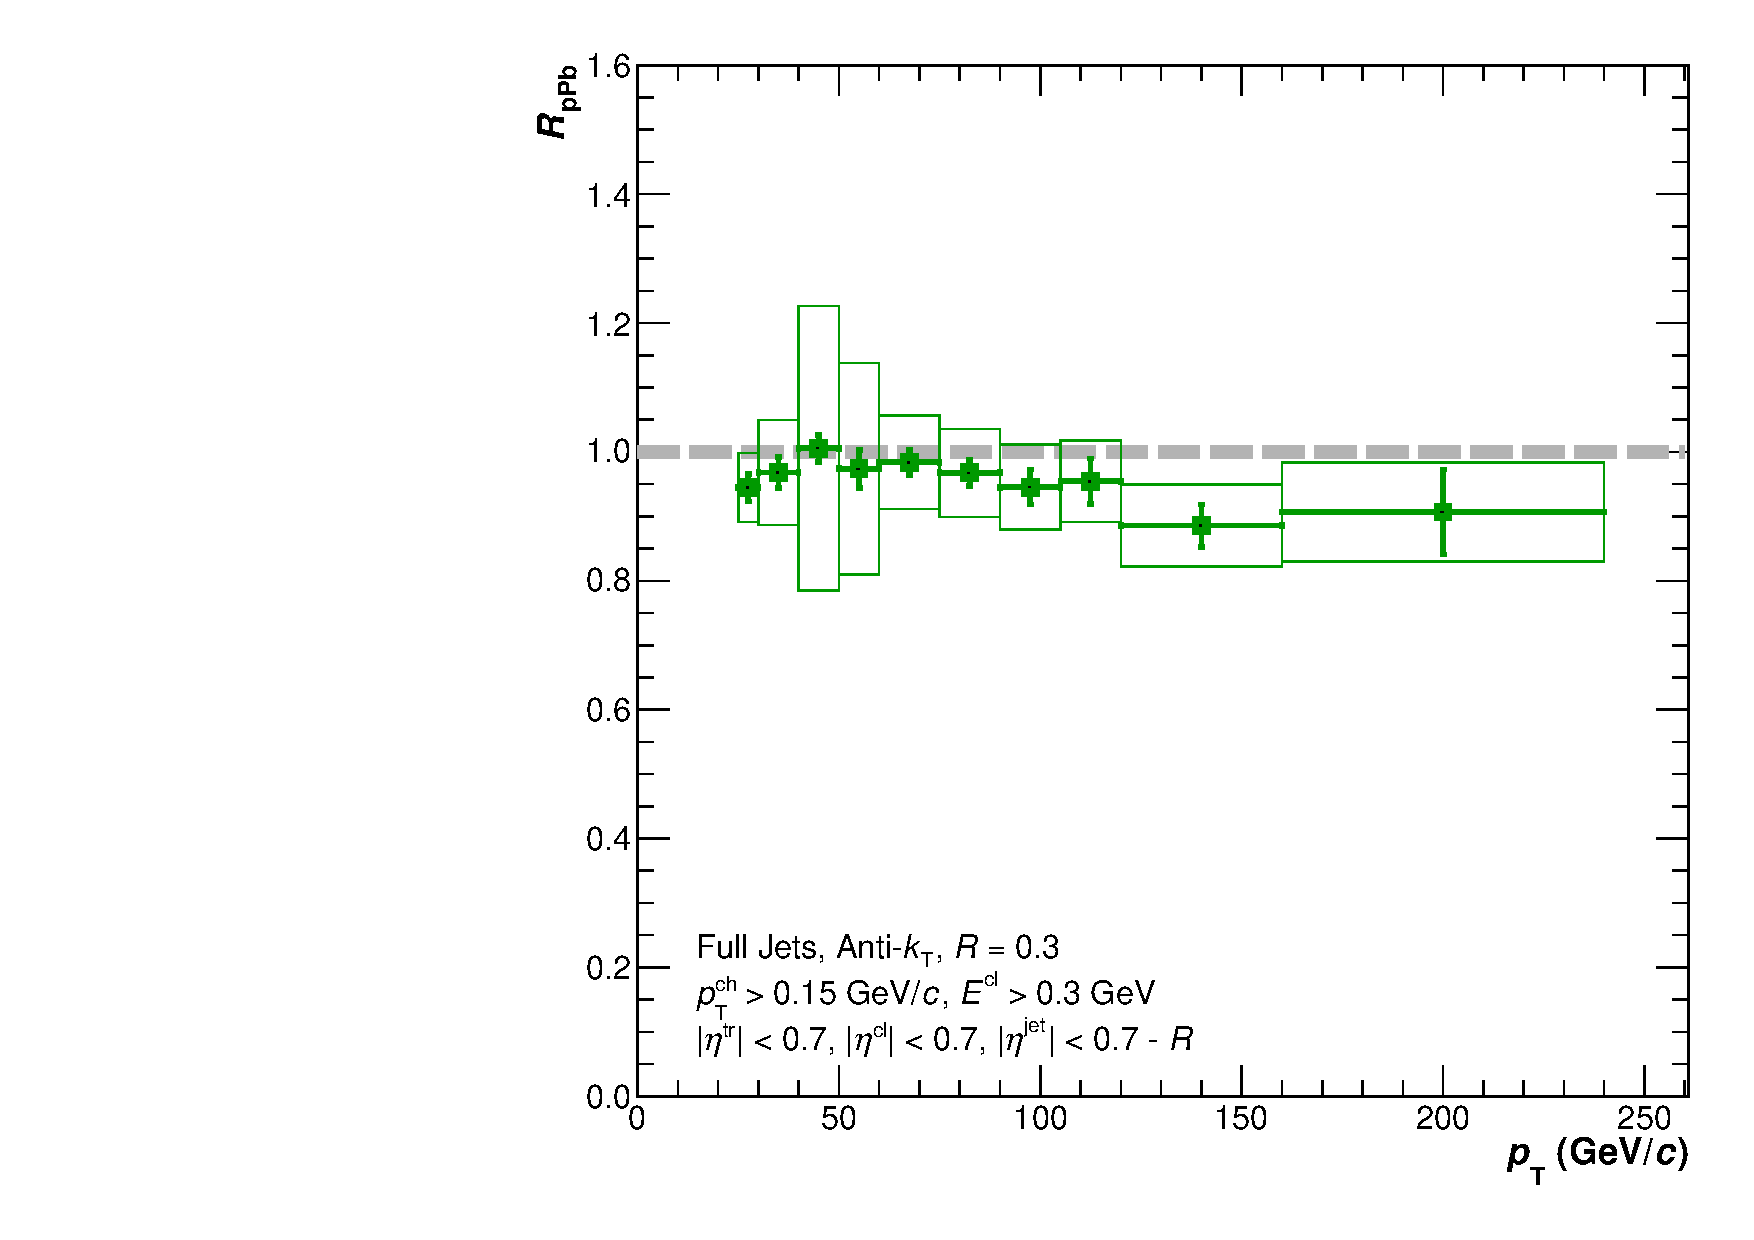
\includegraphics[width=0.49\textwidth]{figures/pPbFigures/RpPb/ptscheme/RpPb_R03.pdf}
    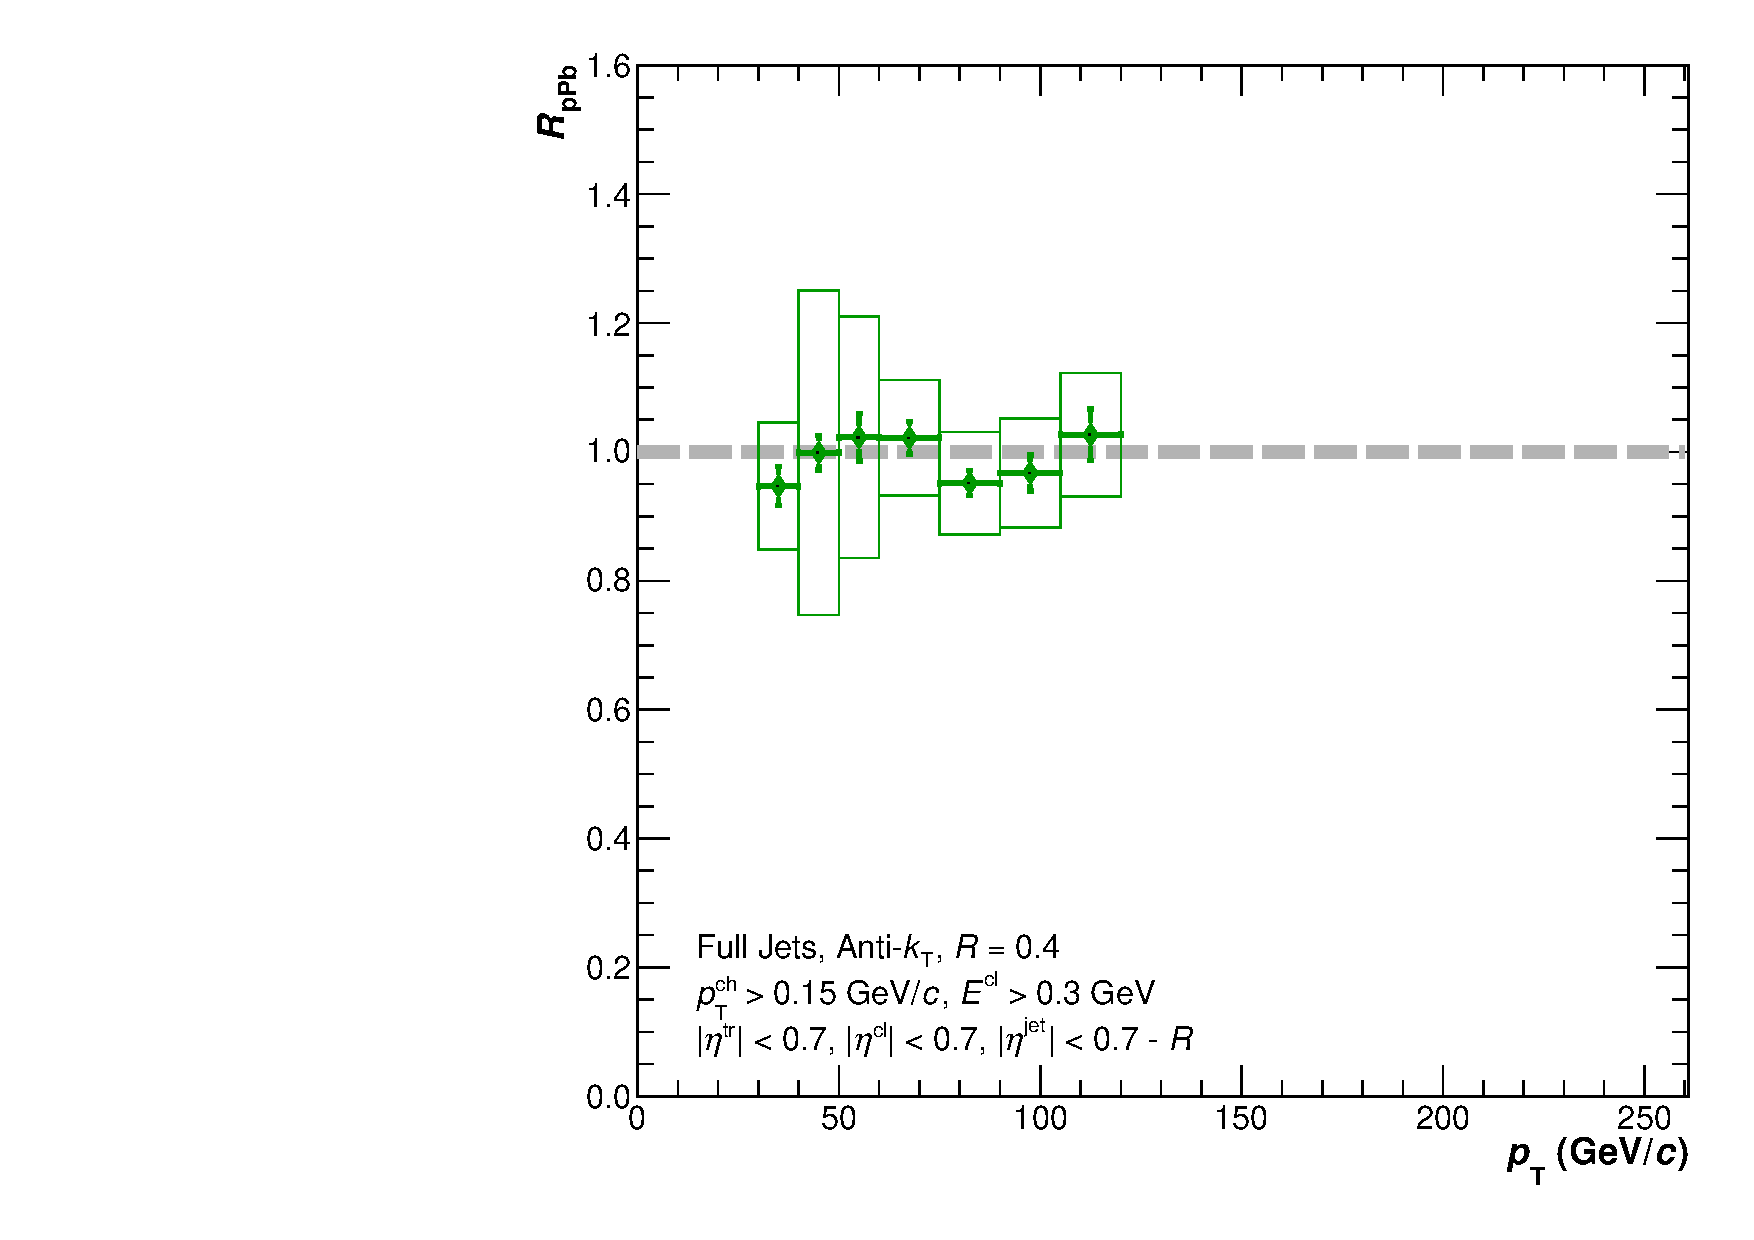
\includegraphics[width=0.49\textwidth]{figures/pPbFigures/RpPb/ptscheme/RpPb_R04.pdf}
    \caption{Nuclear modification factor (\RpPb) for R = 0.2 (top left), R = 0.3 (top right), and R = 0.4 (bottom).}
    \label{fig:finalRpPb}
\end{figure}

This is predominantly consistent with previous measurements performed by ALICE, ATLAS, CMS, and PHENIX, shown in Figure~\ref{fig:RpPbComp}; although, the CMS measurement shows a slight enhancement around 100 GeV/c. Since charged particle jets only reconstruct the charged component of the jet, the yields will be shifted down in jet \pT with respect to the equivalent fully reconstructed jet population. The charged jet \RpPb is scaled by 1.5 to approximately account for the difference in jet reconstruction between charged and fully reconstructed jets. Due to higher statistics from the use of EMCal triggers, the uncertainties on fully reconstructed jets are smaller than those on charged particle jets with the exception of the \pT range in the trigger transition region. ALICE measurements of the \RpPb in charged and fully reconstructed jets are in agreement for all resolution parameters.

The \RpPb for resolution parameter $R$ = 0.2 falls slightly below one at high-\pT, suggesting possible suppression for jets with a small resolution parameter at high-\pT. The previous full jet measurements that extend to this kinematic range did not measure jets at resolution parameter $R$ = 0.2, so no claims can be made about agreement.

\begin{figure}[hbt!]
    \centering
    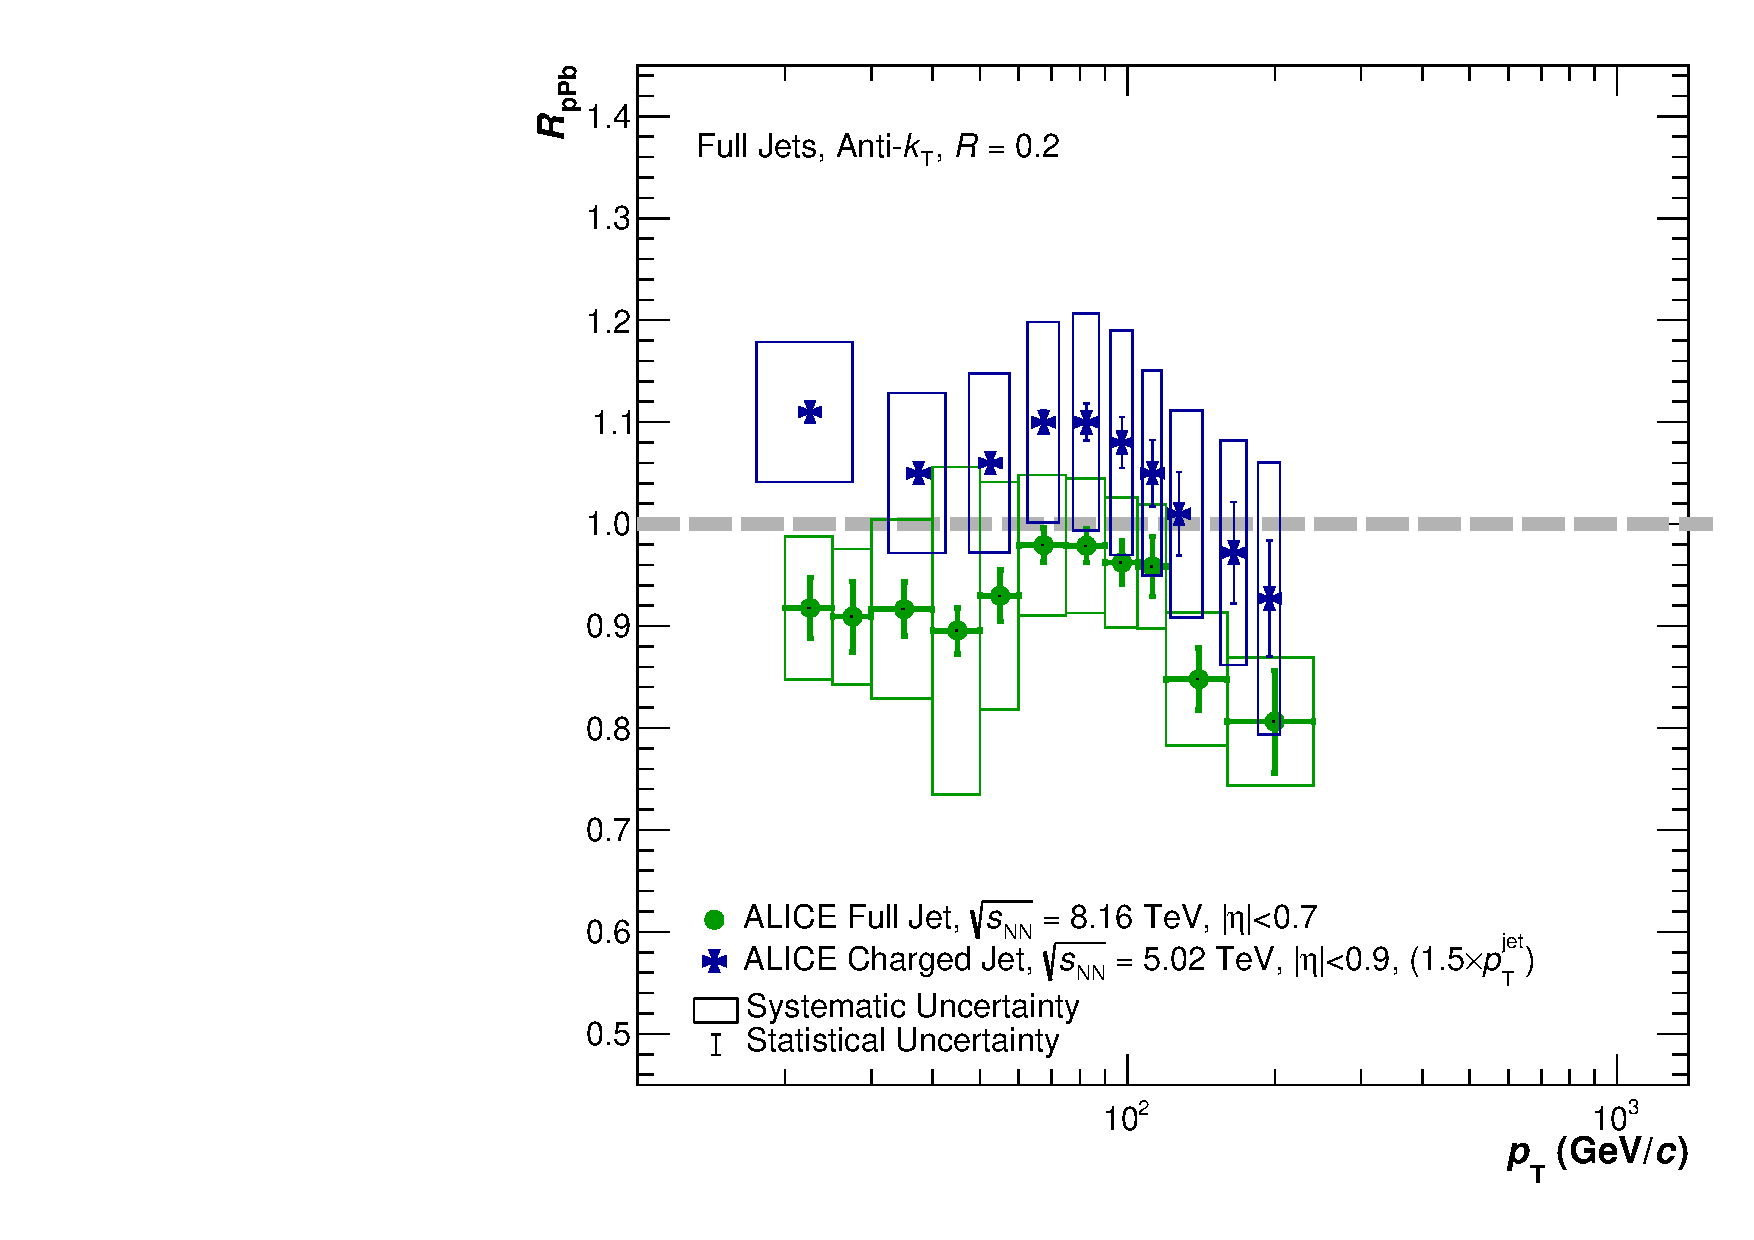
\includegraphics[width=0.49\textwidth]{figures/pPbFigures/RpPb/experimentComp/RpPbCombined_R02.pdf}
    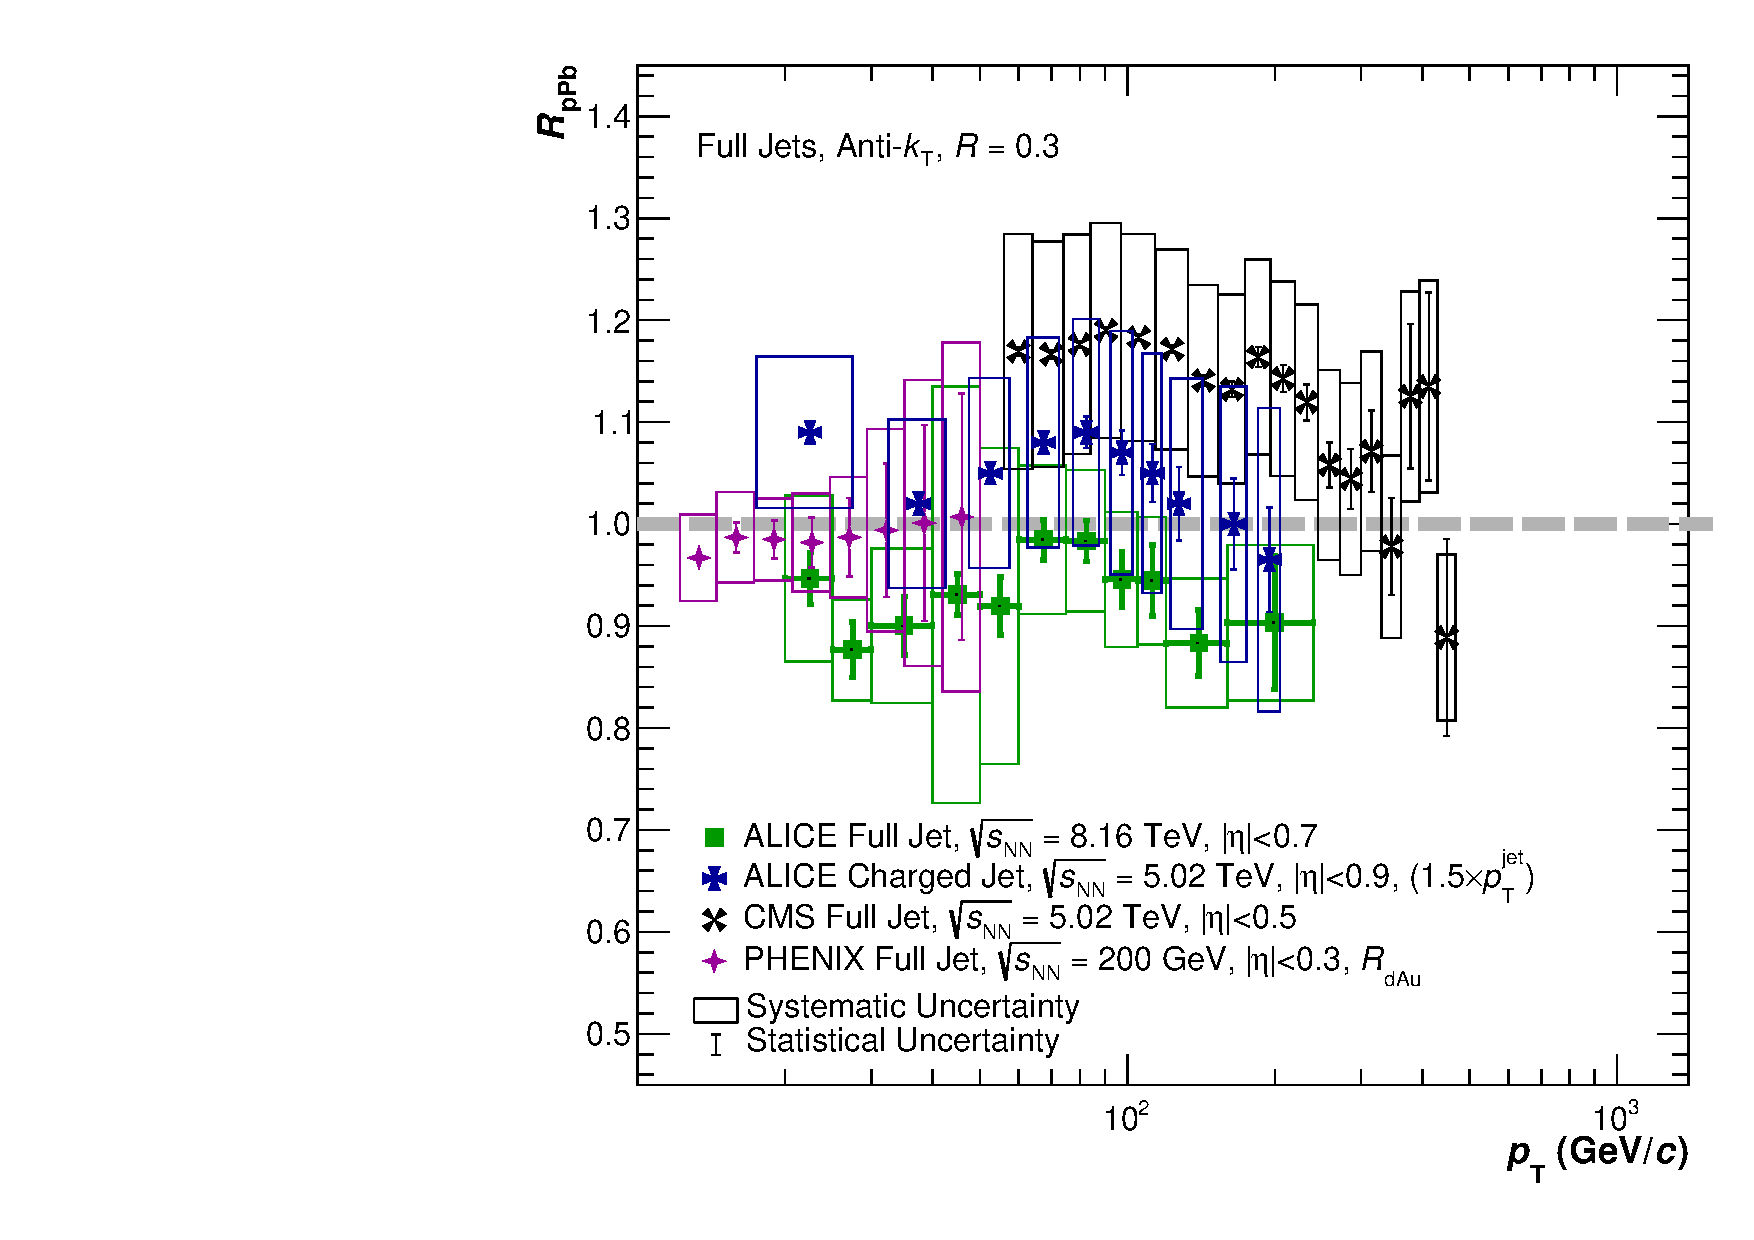
\includegraphics[width=0.49\textwidth]{figures/pPbFigures/RpPb/experimentComp/RpPbCombined_R03.pdf}
    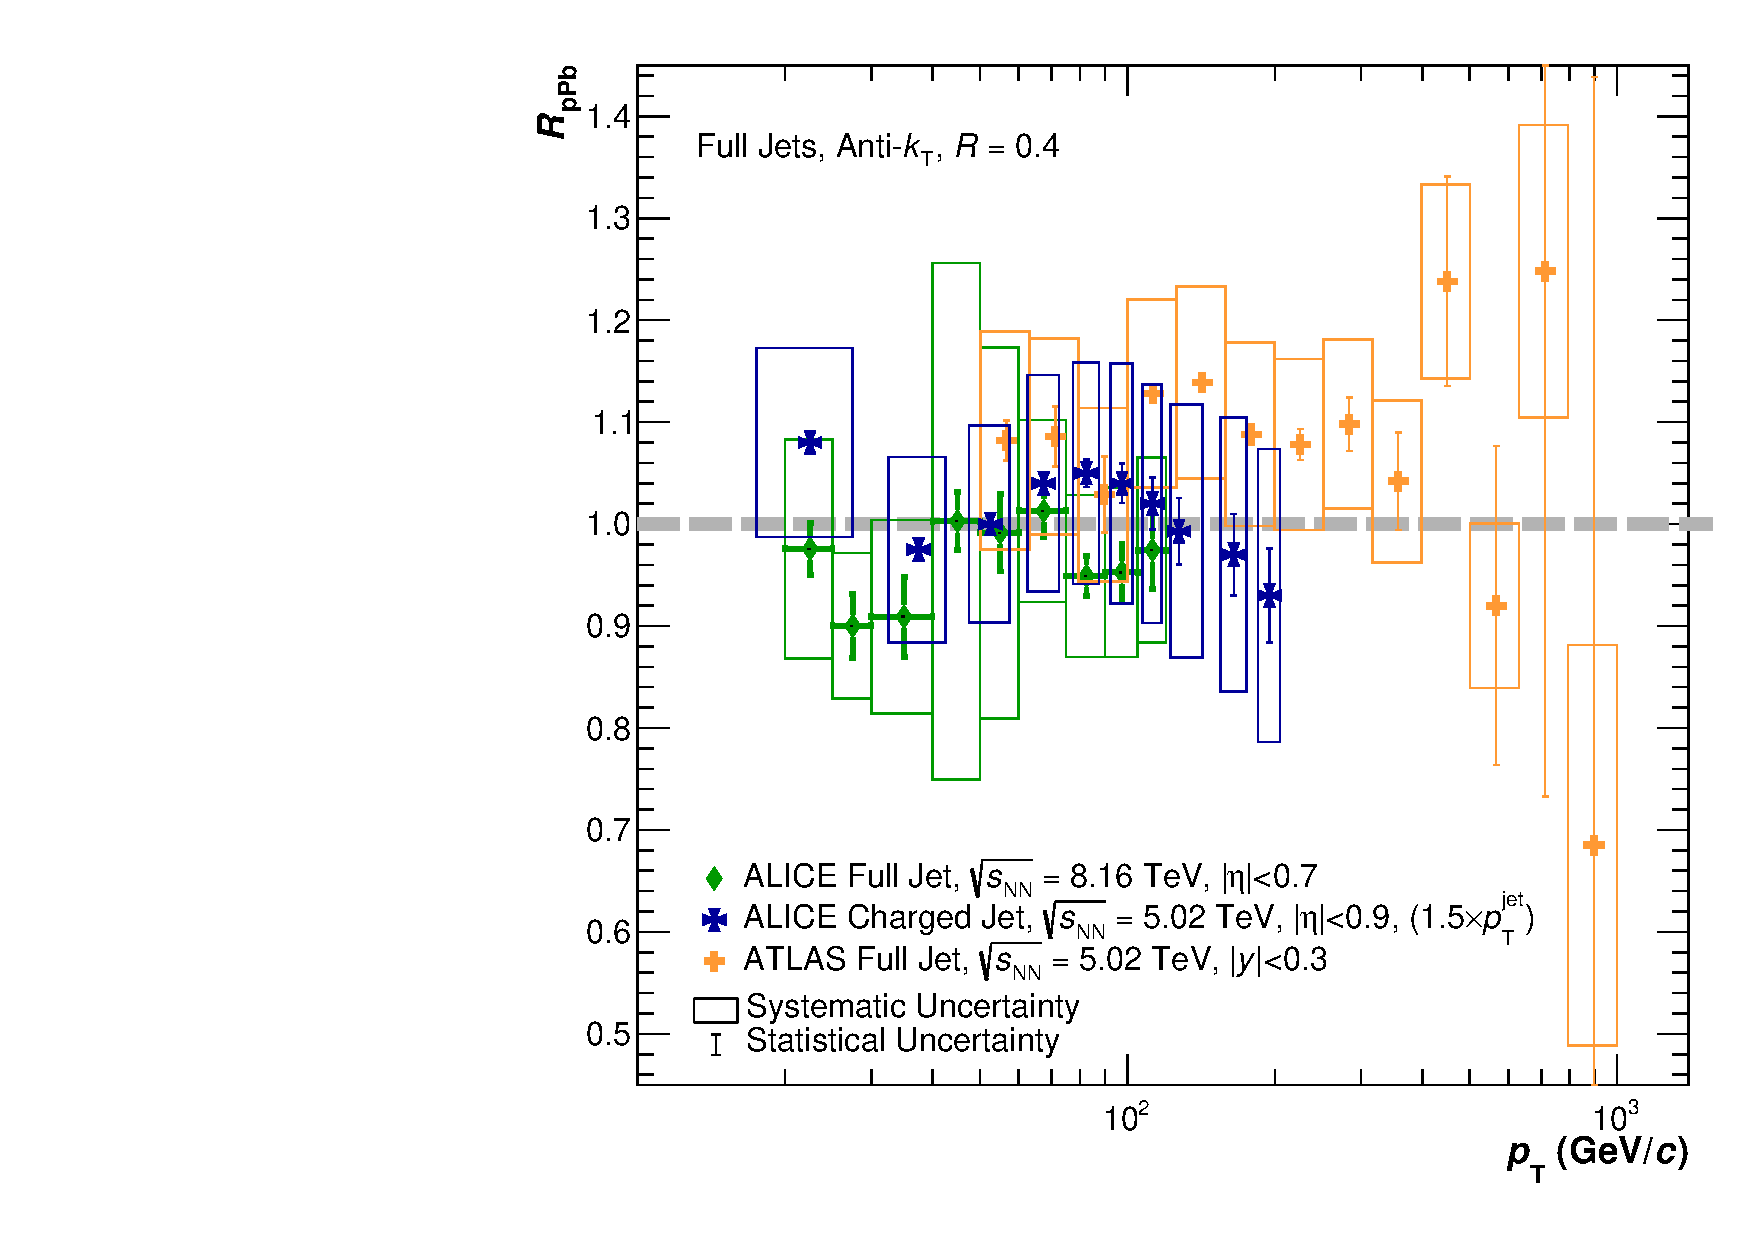
\includegraphics[width=0.49\textwidth]{figures/pPbFigures/RpPb/experimentComp/RpPbCombined_R04.pdf}
    \caption{Comparison of the jet nuclear modification factors \RpPb (ALICE, ATLAS, CMS) and \RdAu (PHENIX) for R = 0.2 (top left), R = 0.3 (top right), and R = 0.4 (bottom). The \pT for charged particle jets in ALICE is scaled by 1.5.}
    \label{fig:RpPbComp}
\end{figure}

Although previous measurements using larger radius fully reconstructed jets showed little to no modification, the work presented here shows a slight suppression of $R$ = 0.2 jets at high-\pT. This observation suggests that the transverse momentum is more spread out in $\eta-\phi$ space in \pPb collisions, and while jets with resolution parameter $R$ = 0.4 or greater recapture the full momentum, small radius jets are sensitive to this modification.

\subsection{Comparison to PYTHIA and POWHEG}
\label{sec:mcComparison}

The jet spectra and ratios in \pp collisions are compared to calculations using PYTHIA8 Monash and POWHEG+PYTHIA8. Fig. \ref{fig:MCGen} shows the comparison of the \pp jet spectra for jet radii R = 0.2 and R = 0.5 to the generator models, and \ref{fig:MCGen_RatioDataMC} shows the ratio of simulation to \pp ALICE data. Fig. \ref{fig:MCGen_Ratio} shows the ratios of radii 0.2/0.3 and 0.2/0.5 compared to the generator models for \pp collisions. It is known that PYTHIA overshoots the \pp data. It has been seen in all collision systems so far, and can also be observed here. POWHEG also overestimates the data, although to a lesser degree.

\begin{figure}
    \centering
    \begin{multicols}{2}
            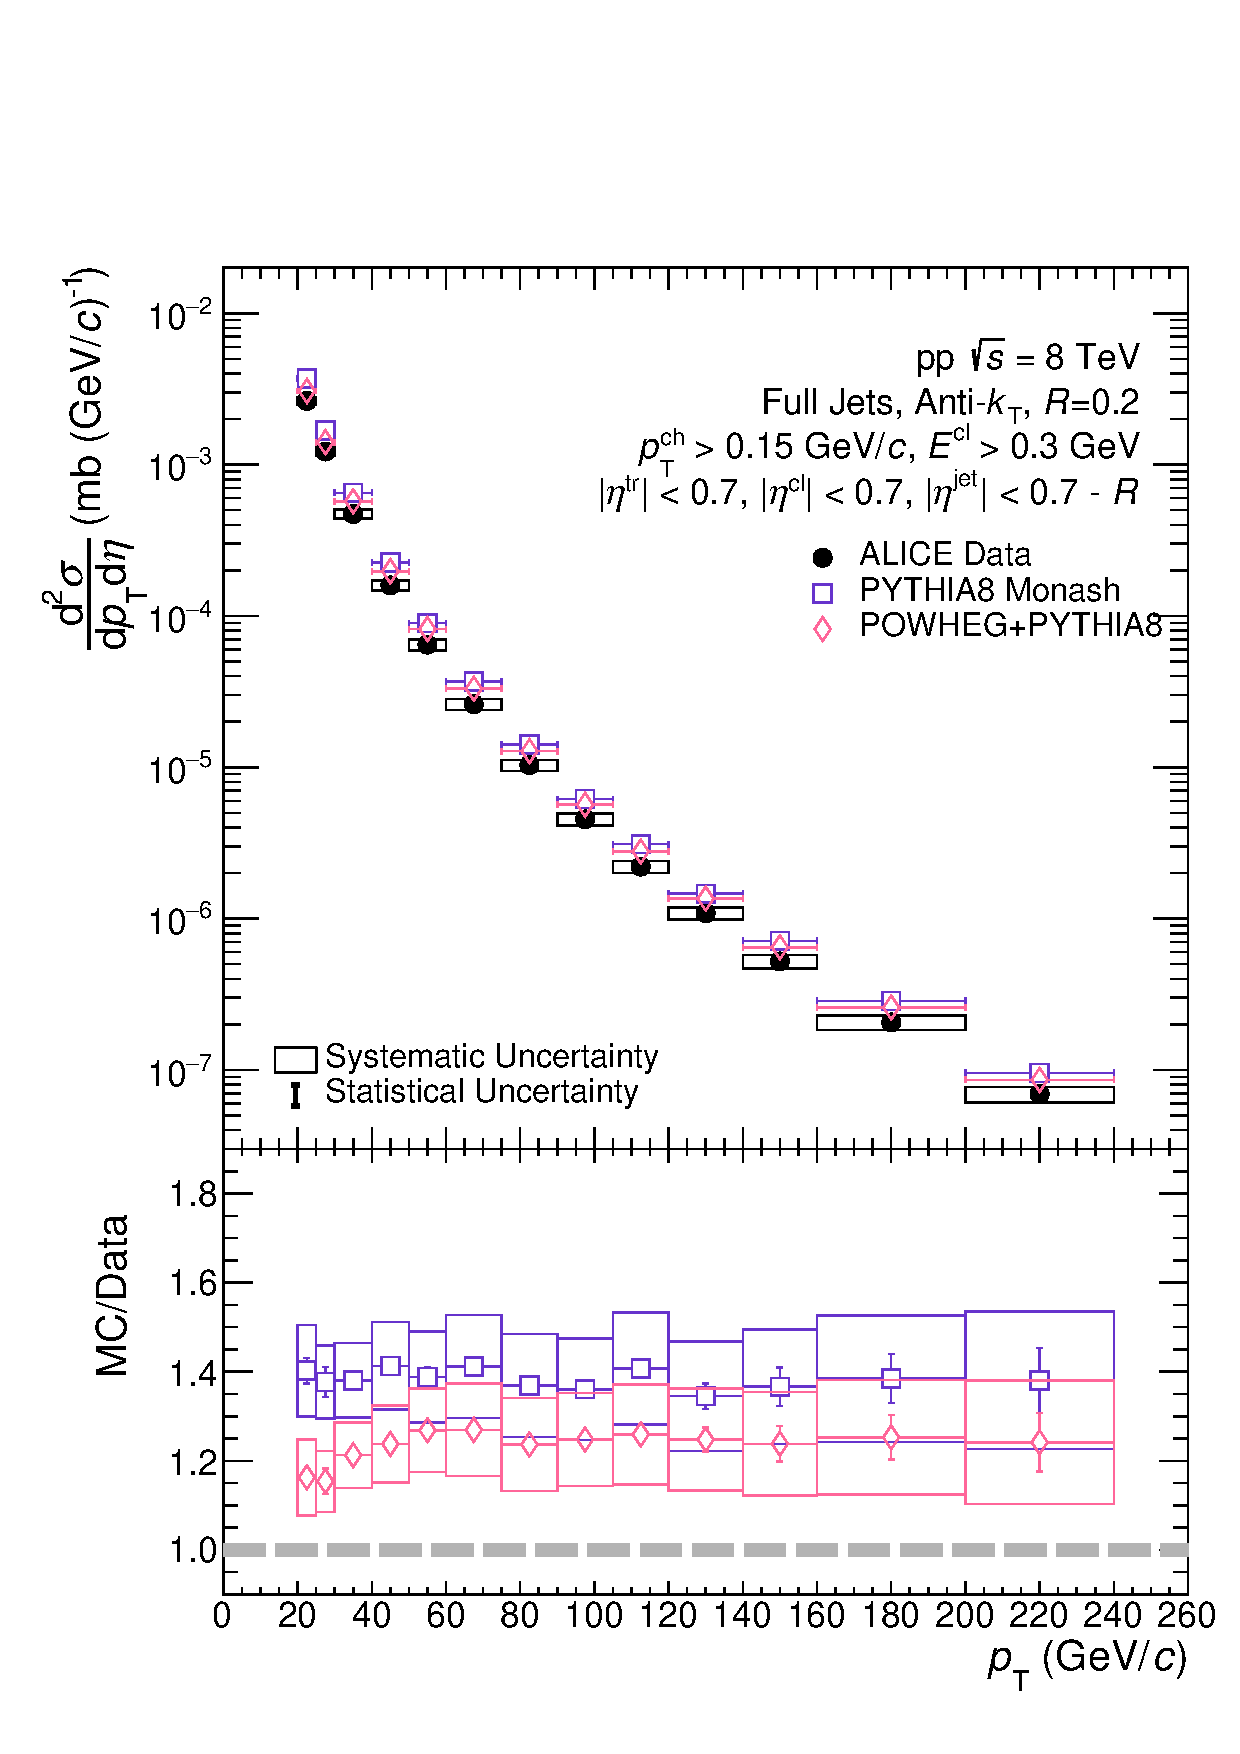
\includegraphics[width=7.5cm]{figures/MCGen/MCComp_R02_nooutlier.pdf}
        \vfill\null
        \columnbreak
            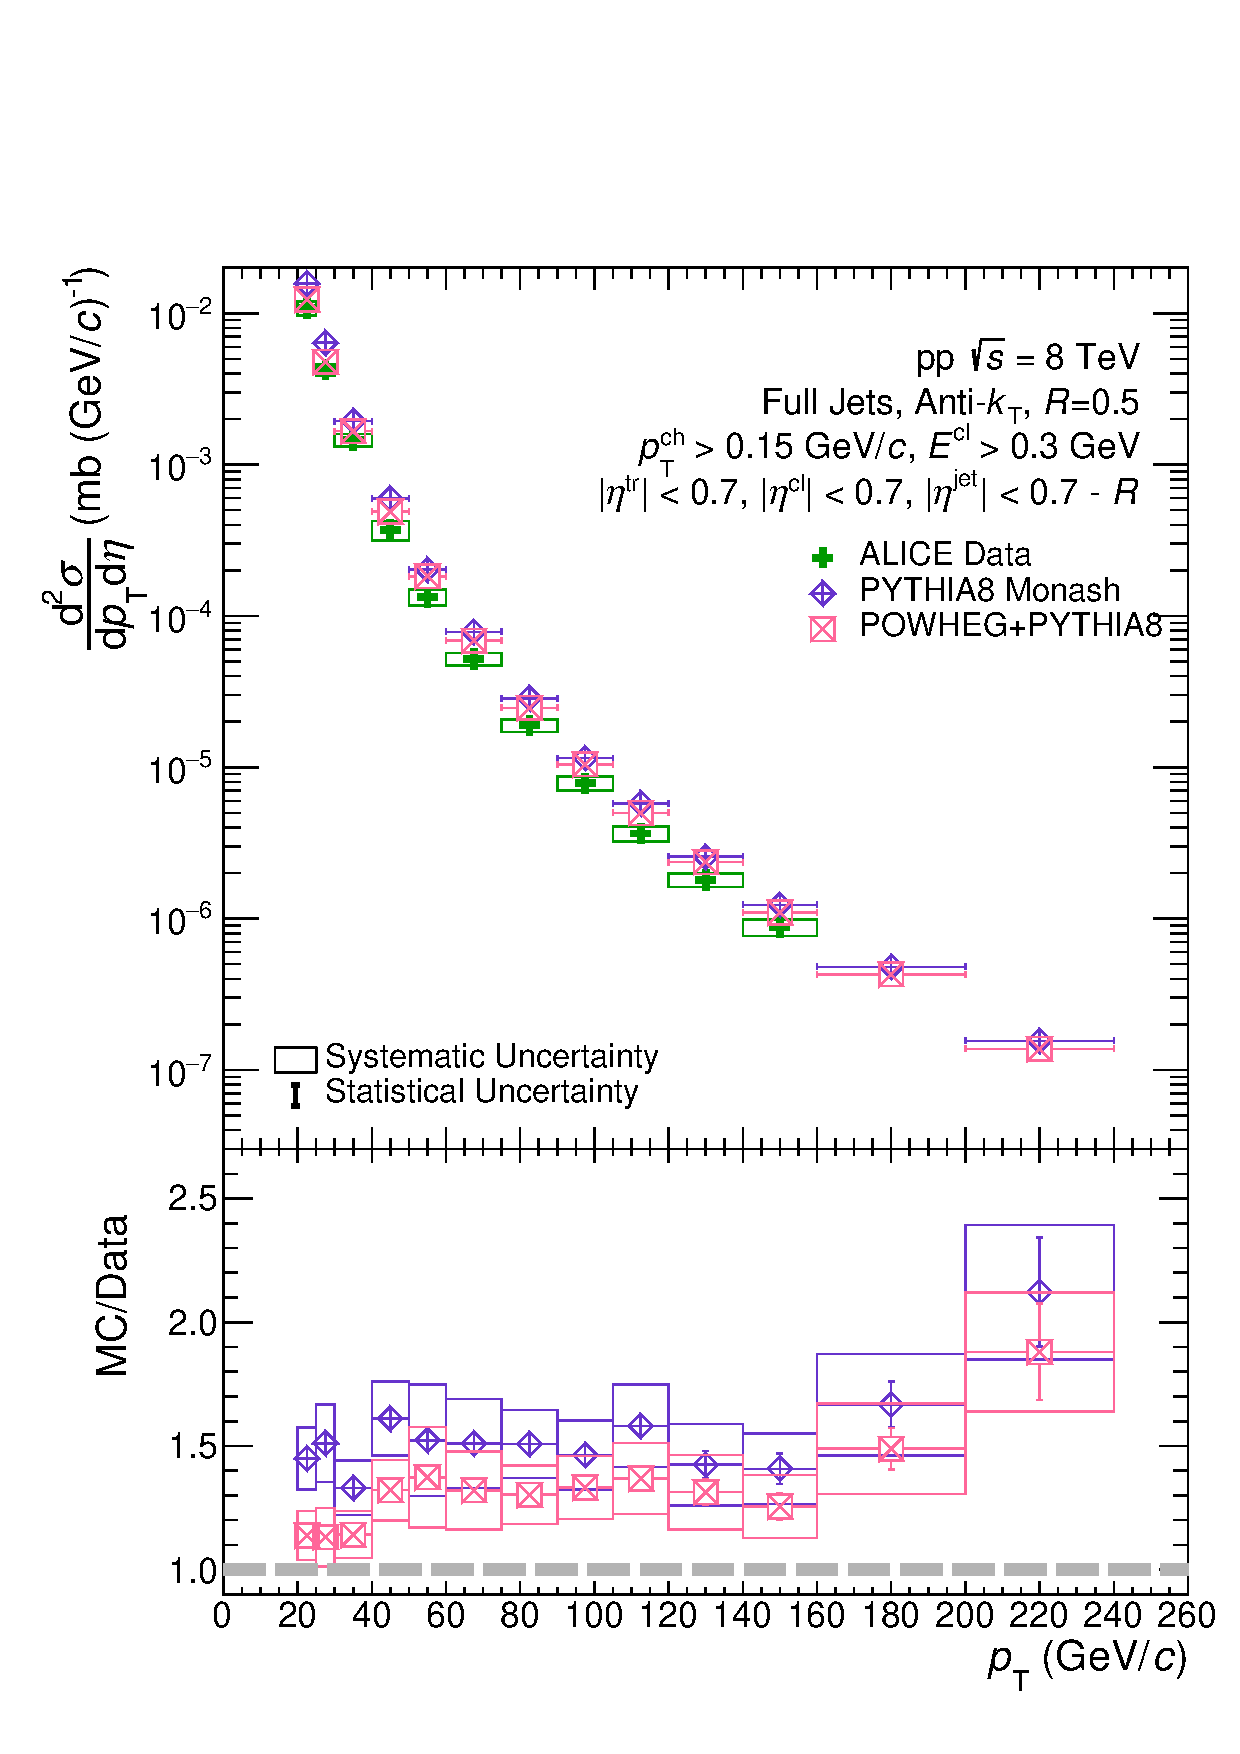
\includegraphics[width=7.5cm]{figures/MCGen/MCComp_R05_nooutlier.pdf}
        \vfill\null
    \end{multicols}
    \caption{Comparison to PYTHIA8 Monash and POWHEG+PYTHIA8 for jet radii 0.2 and 0.5 in \pp collisions.}
    \label{fig:MCGen}
\end{figure}

\begin{figure}
    \centering
    \begin{multicols}{2}
            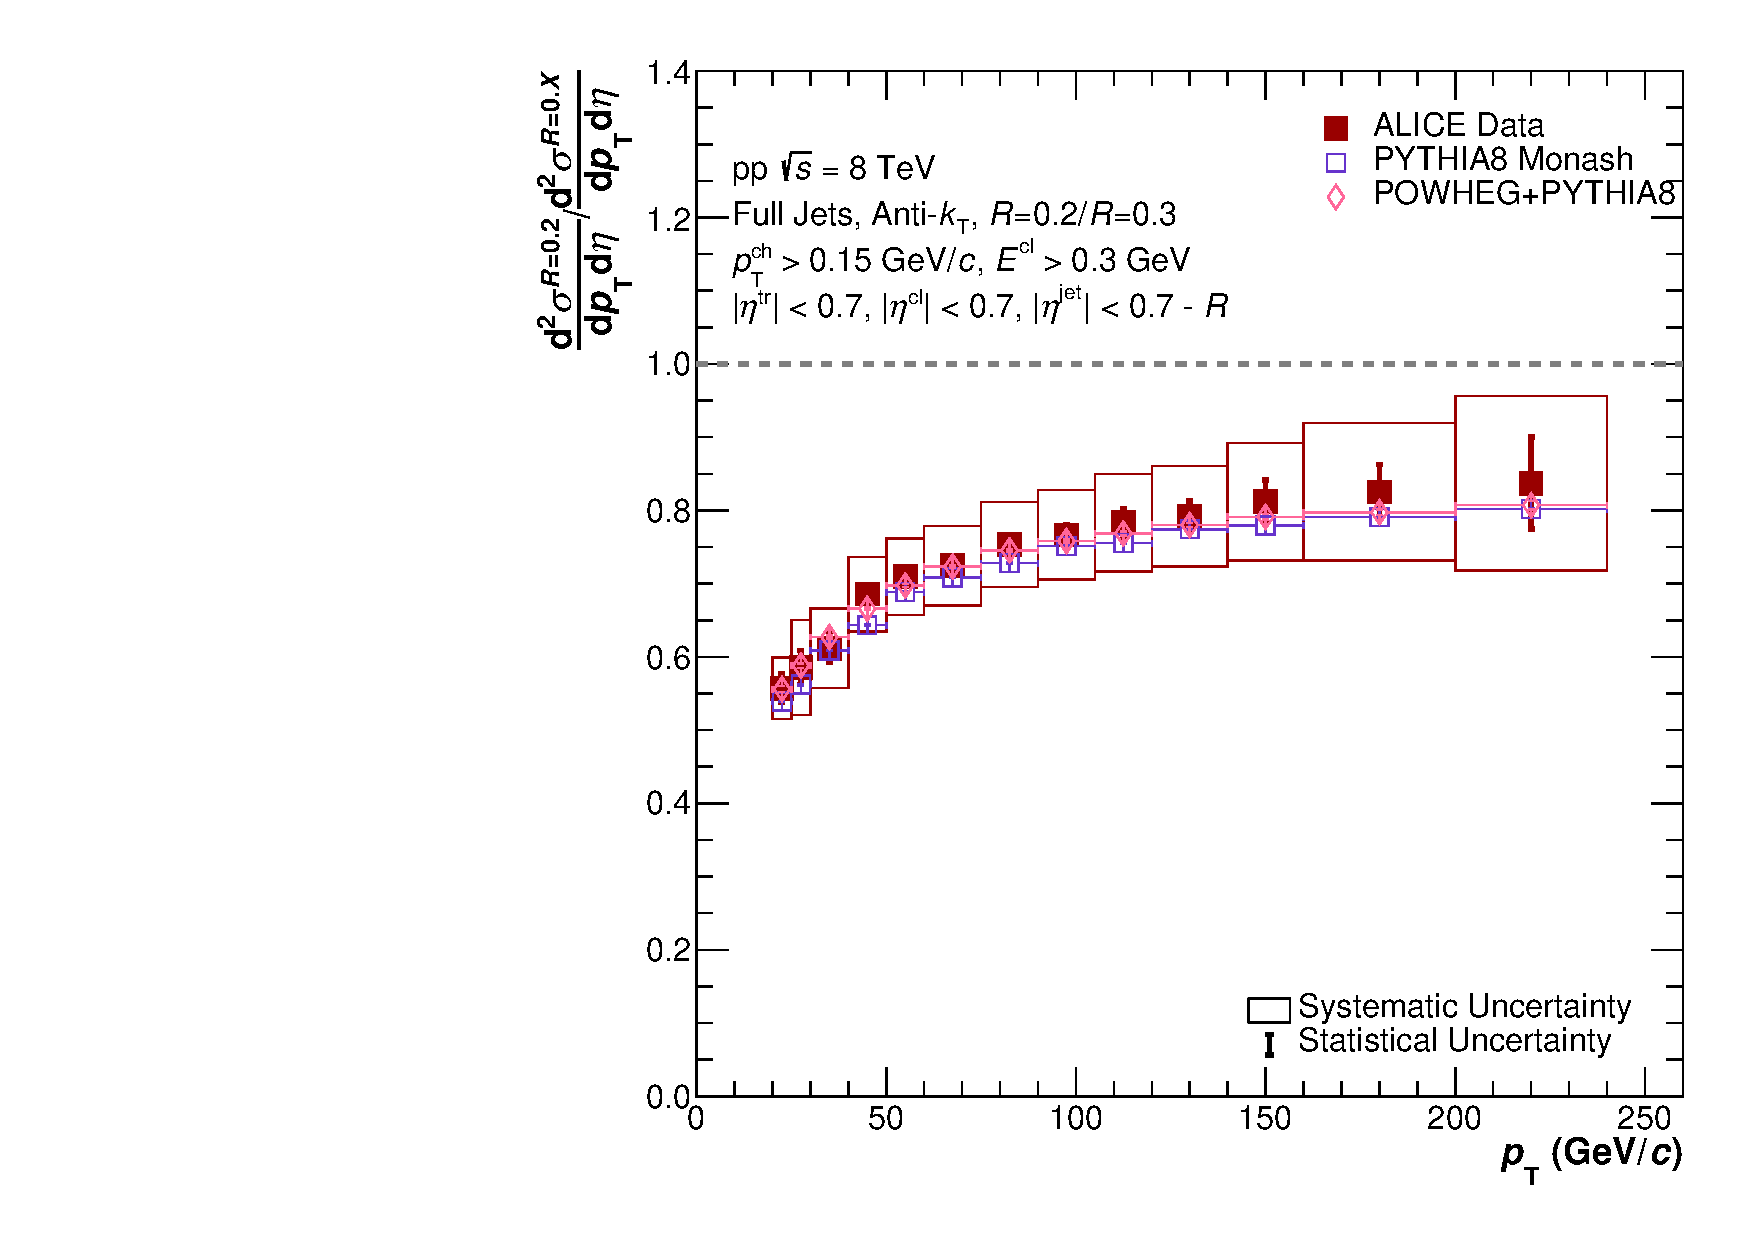
\includegraphics[width=7.5cm]{figures/MCGen/MCComp_Ratio_R0302_nooutlier.pdf}
        \vfill\null
        \columnbreak
            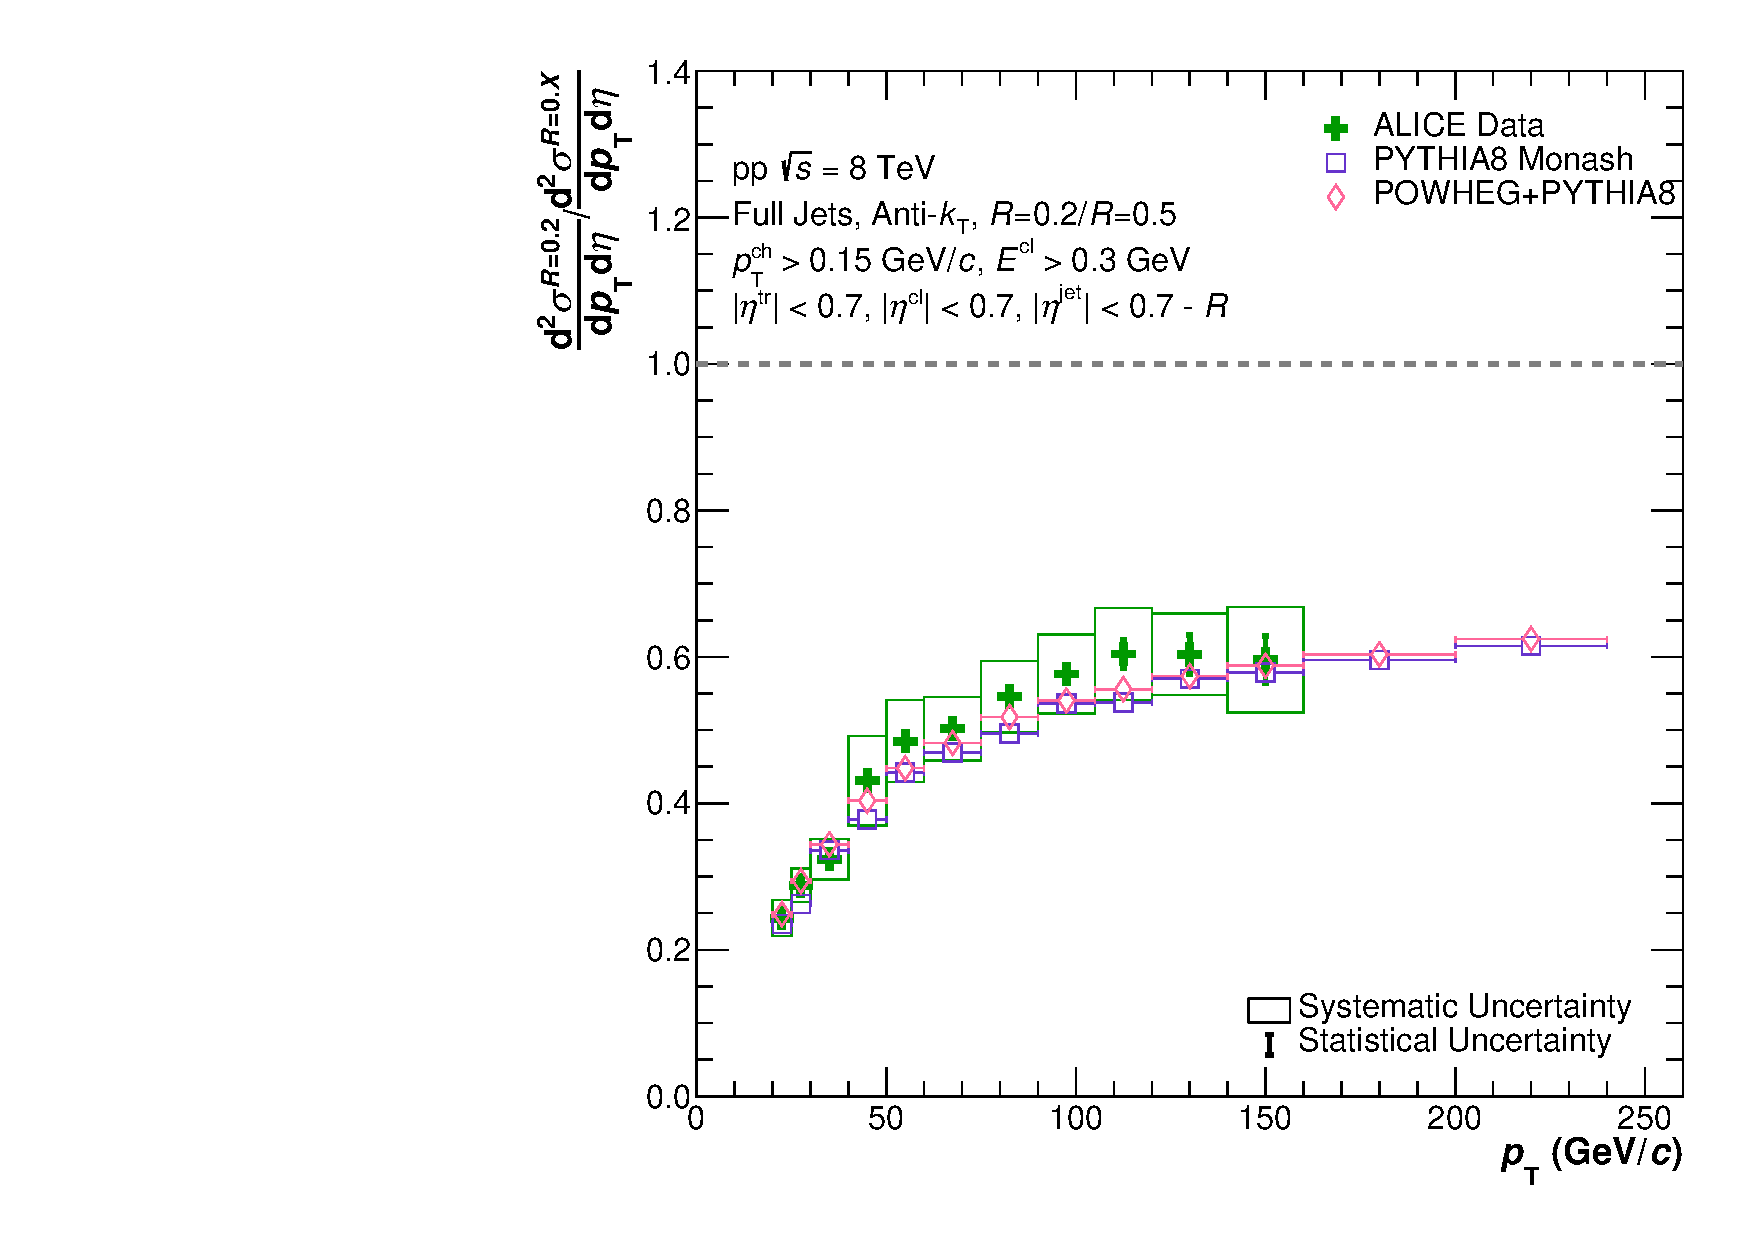
\includegraphics[width=7.5cm]{figures/MCGen/MCComp_Ratio_R0502_nooutlier.pdf}
        \vfill\null
    \end{multicols}
    \caption{Comparison to PYTHIA8 Monash and POWHEG+PYTHIA8 for ratios of jet radii 0.2/0.3 and 0.2/0.5 in \pp collisions.}
    \label{fig:MCGen_Ratio}
\end{figure}

\begin{figure}
    \centering
    \begin{multicols}{2}
            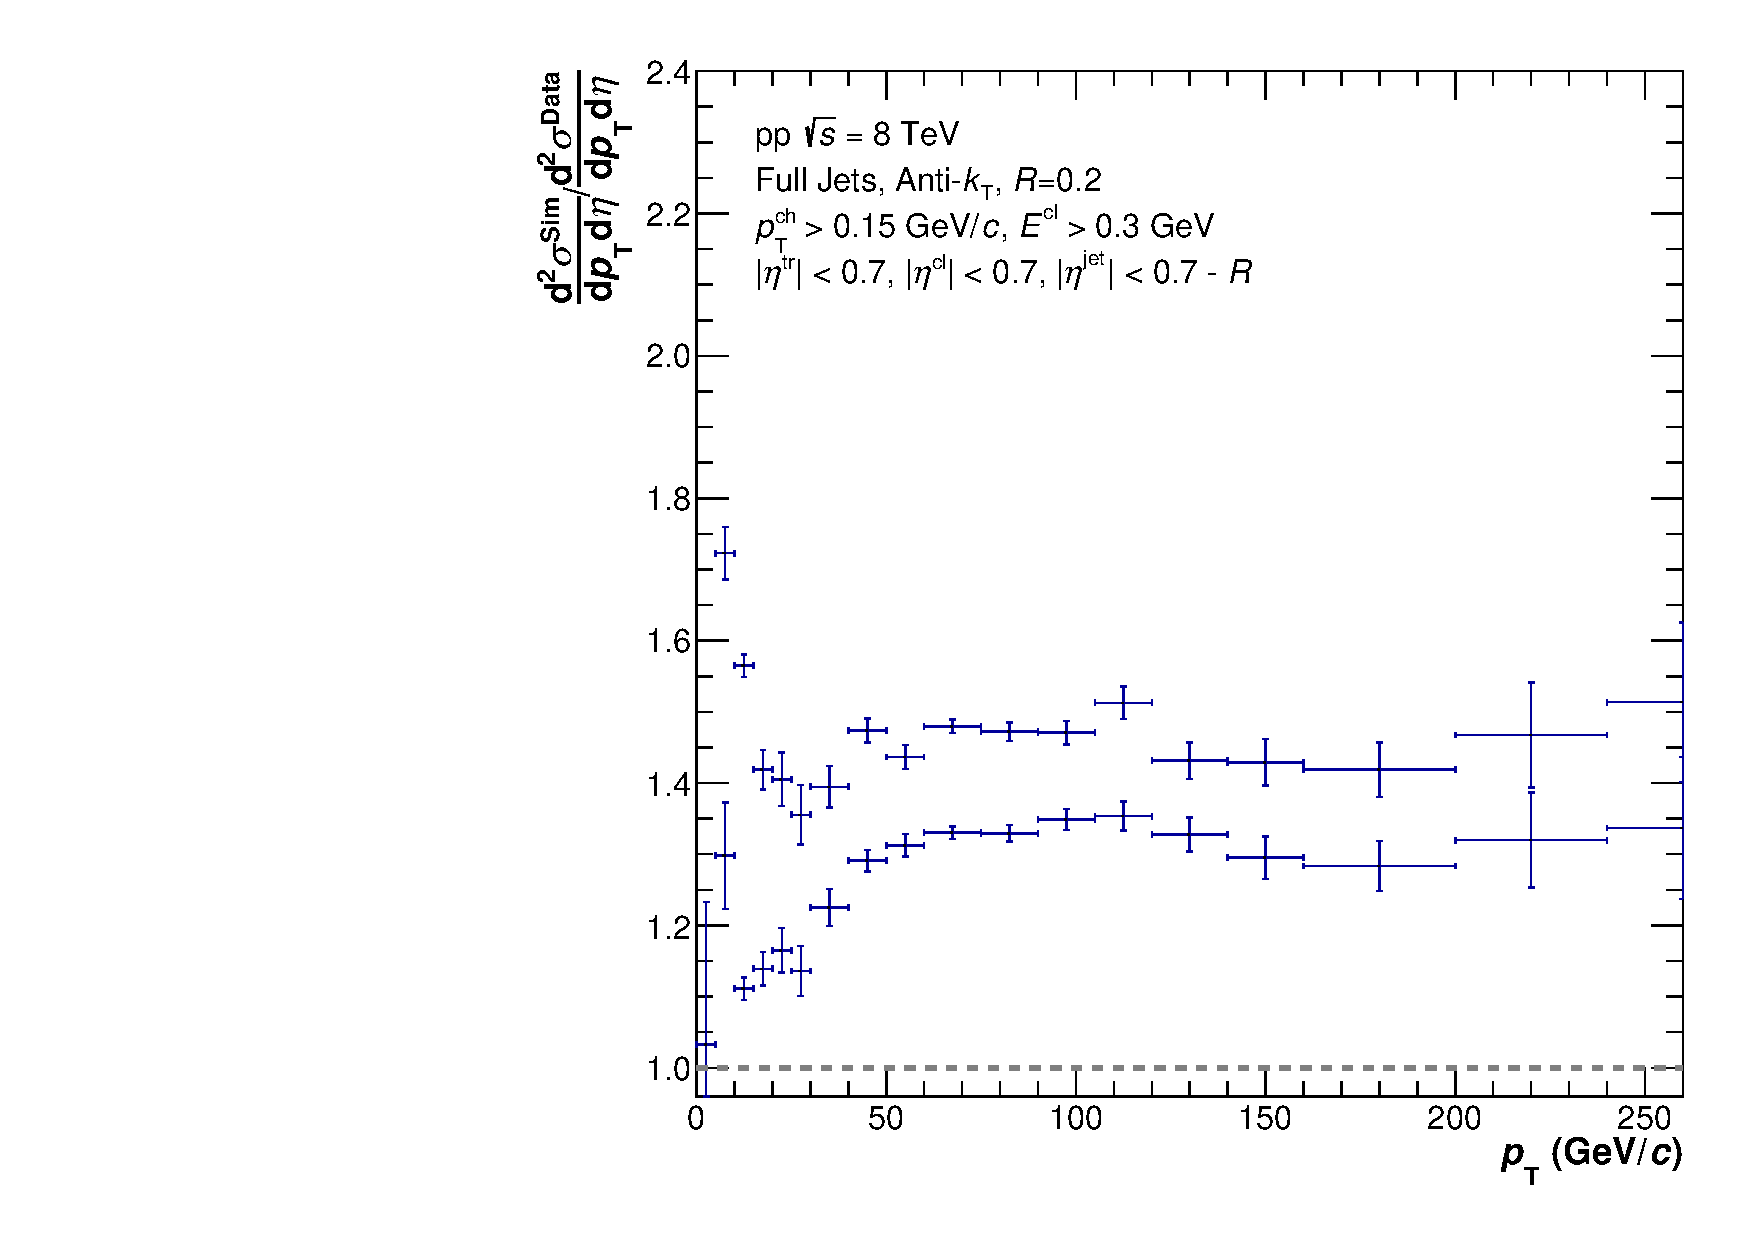
\includegraphics[width=7.5cm]{figures/MCGen/ratioDataMC/ratio_simdata_R02_nooutlier.pdf}
        \vfill\null
        \columnbreak
            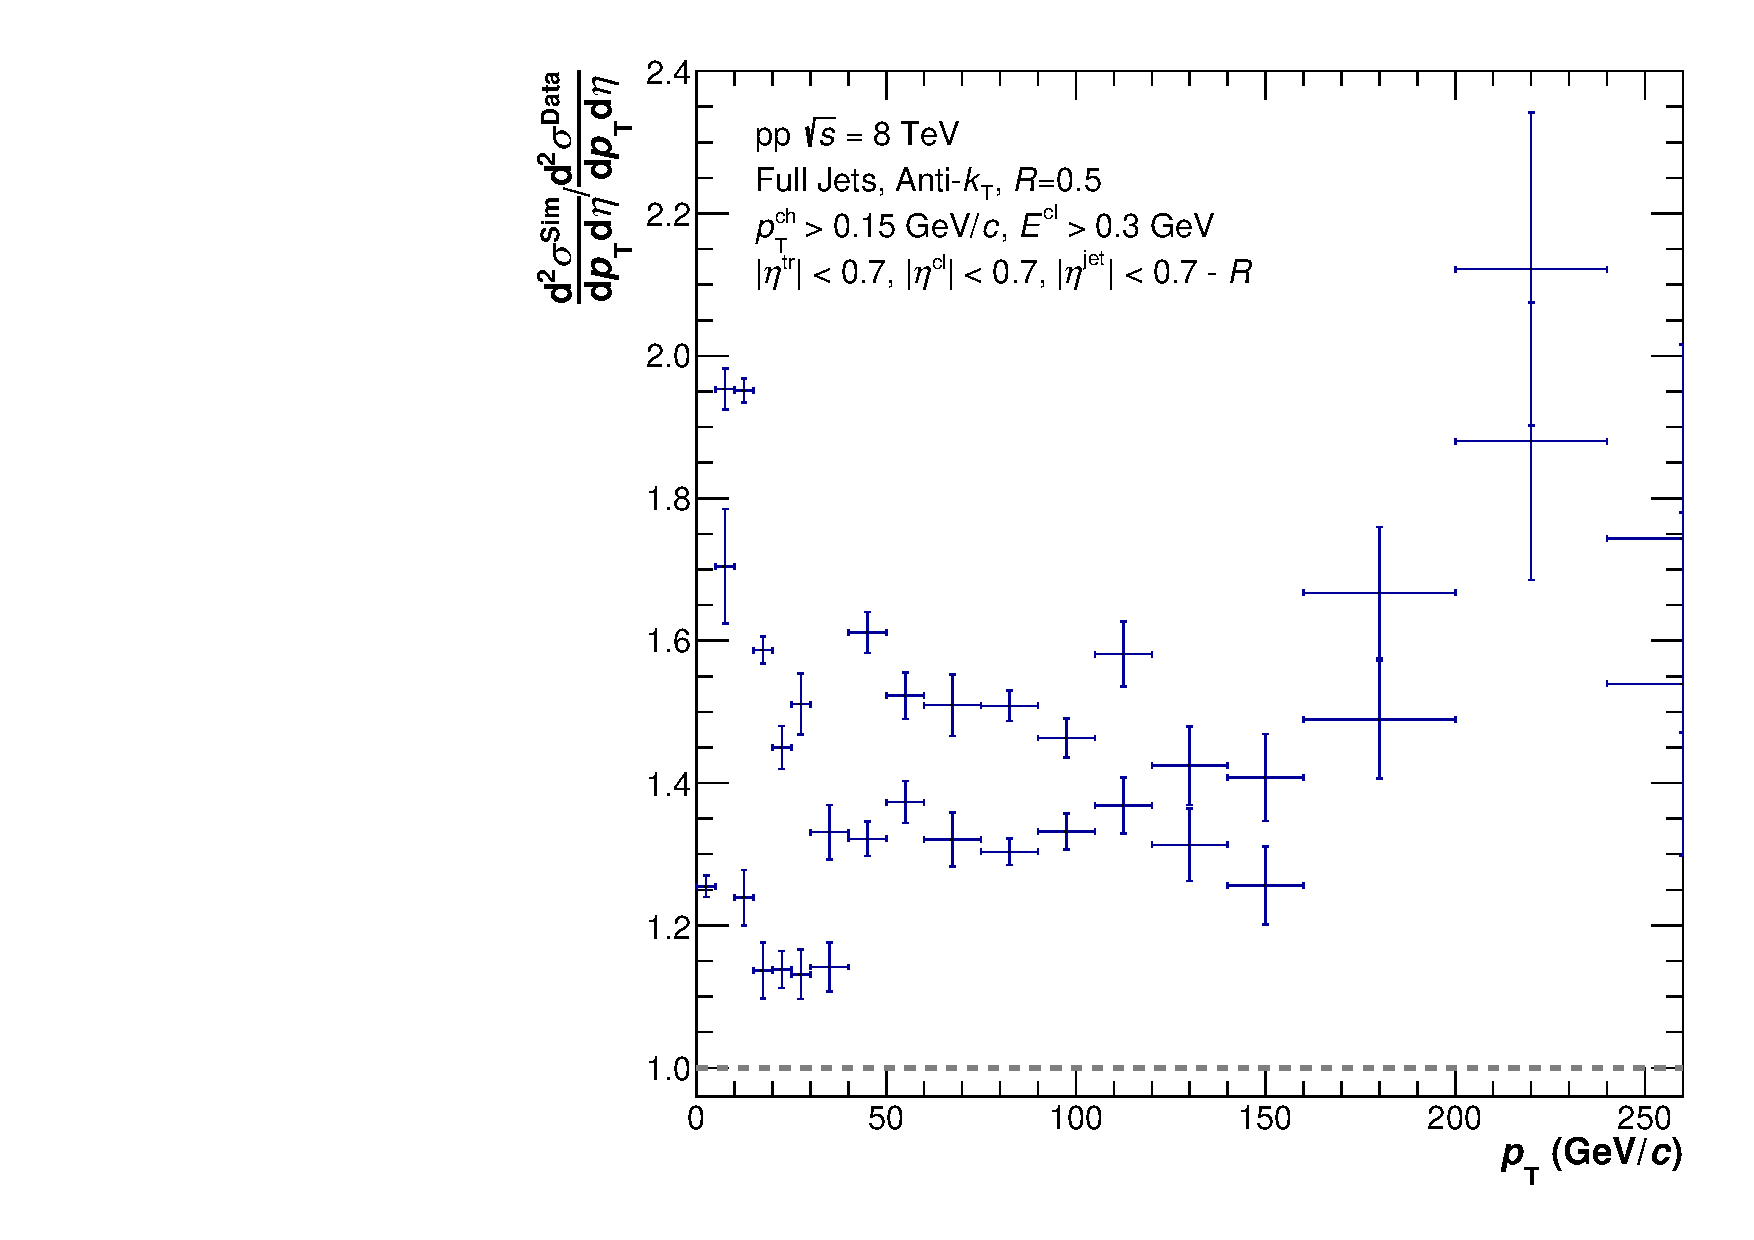
\includegraphics[width=7.5cm]{figures/MCGen/ratioDataMC/ratio_simdata_R05_nooutlier.pdf}
        \vfill\null
    \end{multicols}
    \caption{Ratio of PYTHIA8 Monash and POWHEG+PYTHIA8 to ALICE data for jet radii 0.2 and 0.5 in \pp collisions.}
    \label{fig:MCGen_RatioDataMC}
\end{figure}

Additionally, the jet spectra and ratios in \pPb collisions are compared to calculations using PYTHIA8 Monash and POWHEG+PYTHIA8. PYTHIA8 simulates \pp collisions, and a nuclear PDF was not used for the POWHEG production. Thus, both simulate only \pp collisions. In addition, PYTHIA does not take into account the rapidity shift that is present in data. Fig. \ref{fig:MCGen_pPb} shows the comparison of the \pPb jet spectra for jet radii R = 0.2 and R = 0.5 to the generator models, and \ref{fig:MCGen_RatioDataMC_pPb} shows the ratio of simulation to \pPb ALICE data. Fig. \ref{fig:MCGen_Ratio_pPb} shows the ratios of radii 0.2/0.3 and 0.2/0.5 compared to the generator models for \pPb collisions. 

\begin{figure}
    \centering
    \begin{multicols}{2}
            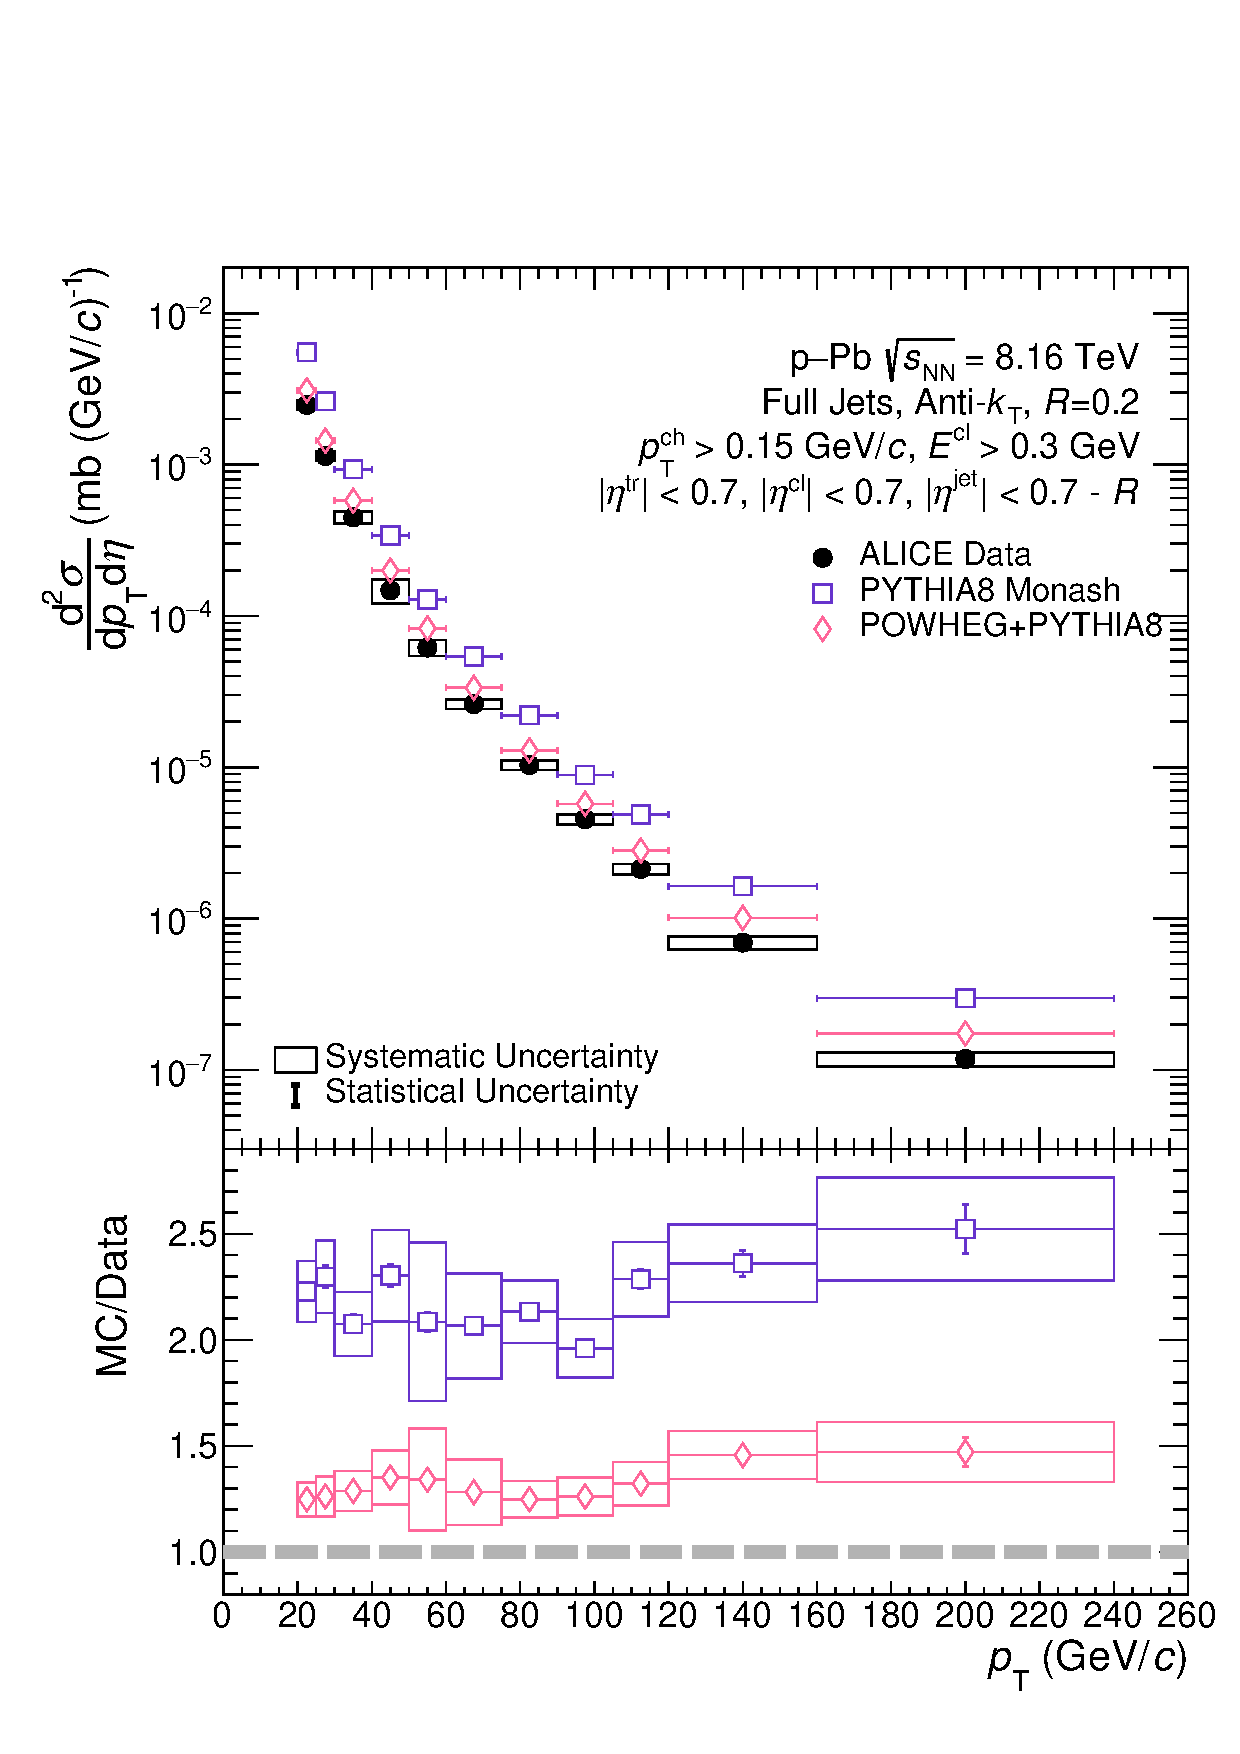
\includegraphics[width=7.5cm]{figures/pPbFigures/MCGen/MCComp_R02_nooutlier.pdf}
        \vfill\null
        \columnbreak
            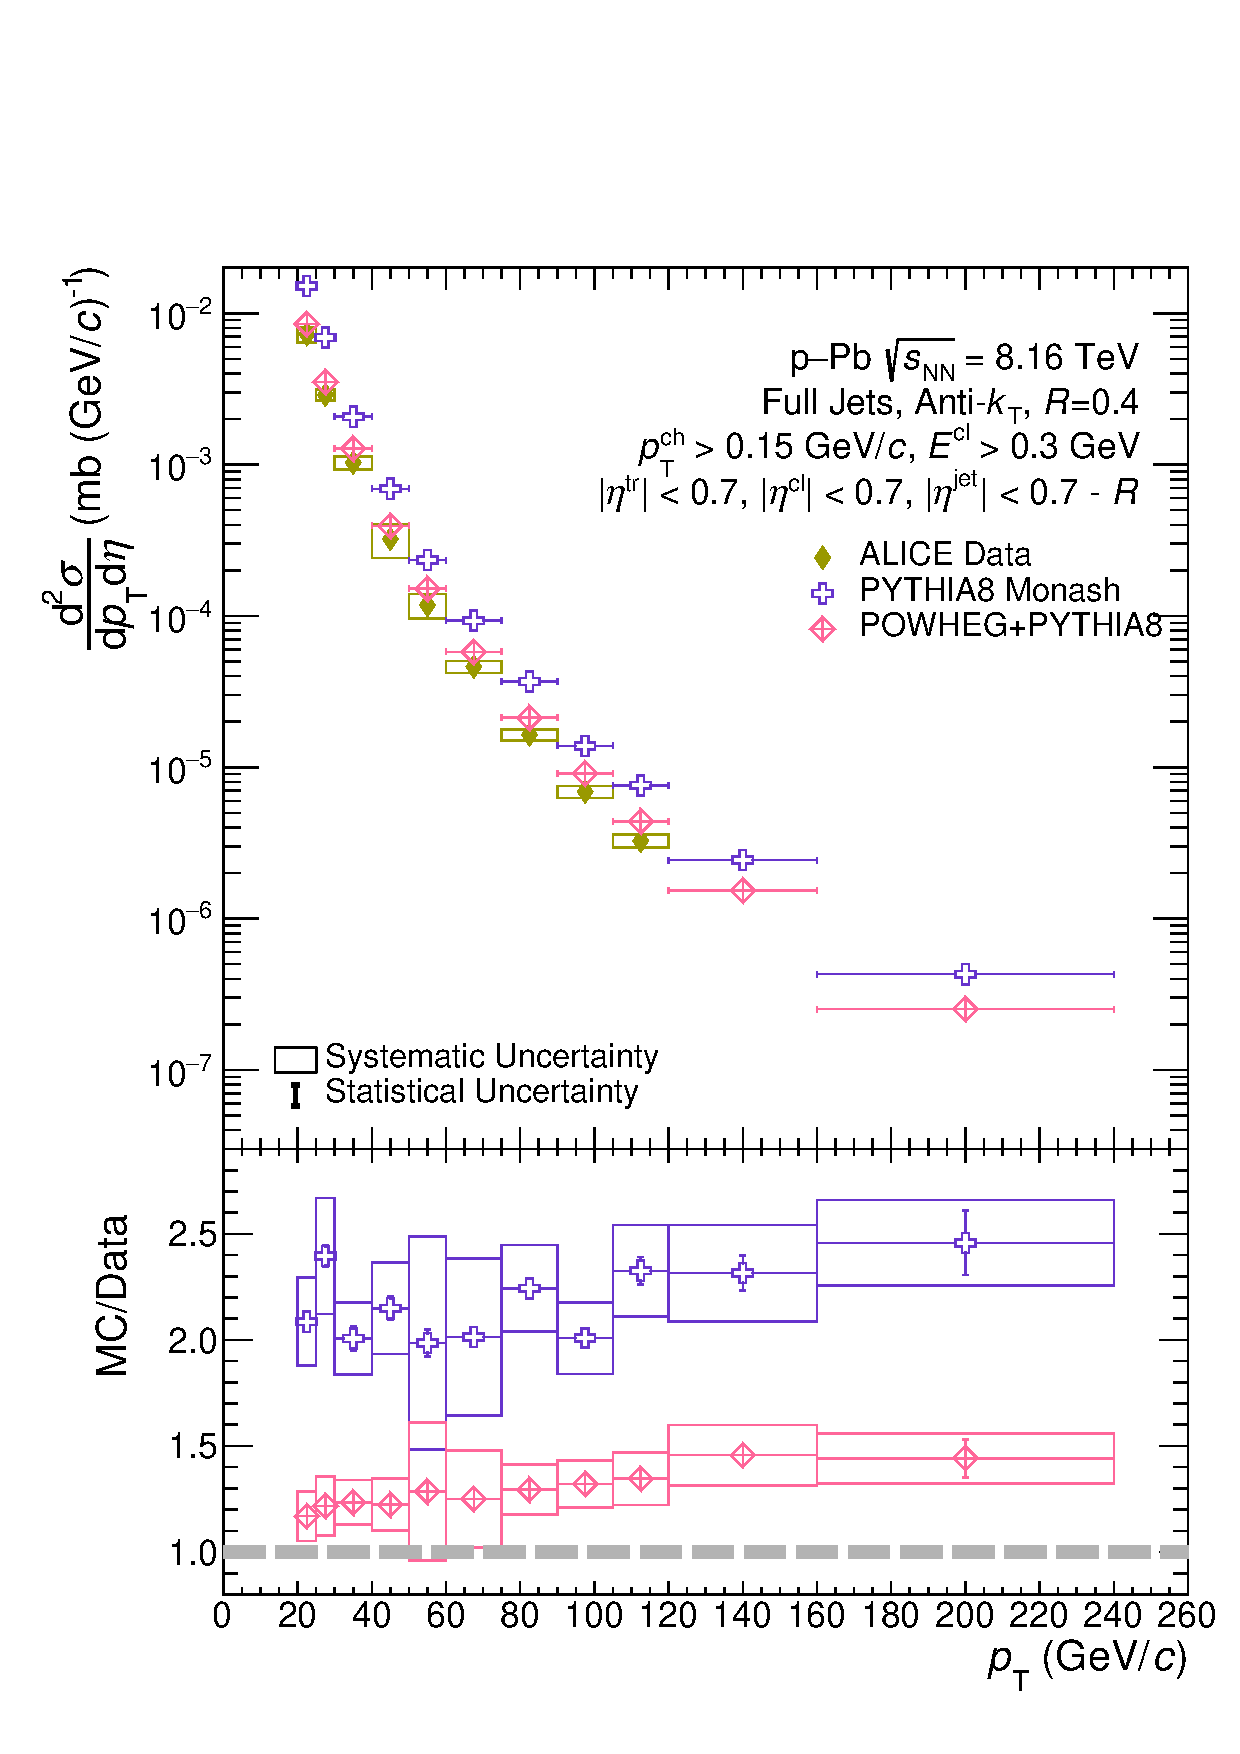
\includegraphics[width=7.5cm]{figures/pPbFigures/MCGen/MCComp_R04_nooutlier.pdf}
        \vfill\null
    \end{multicols}
    \caption{Comparison to PYTHIA8 Monash and POWHEG+PYTHIA8 for jet radii 0.2 and 0.4 in \pPb collisions.}
    \label{fig:MCGen_pPb}
\end{figure}

\begin{figure}
    \centering
    \begin{multicols}{2}
            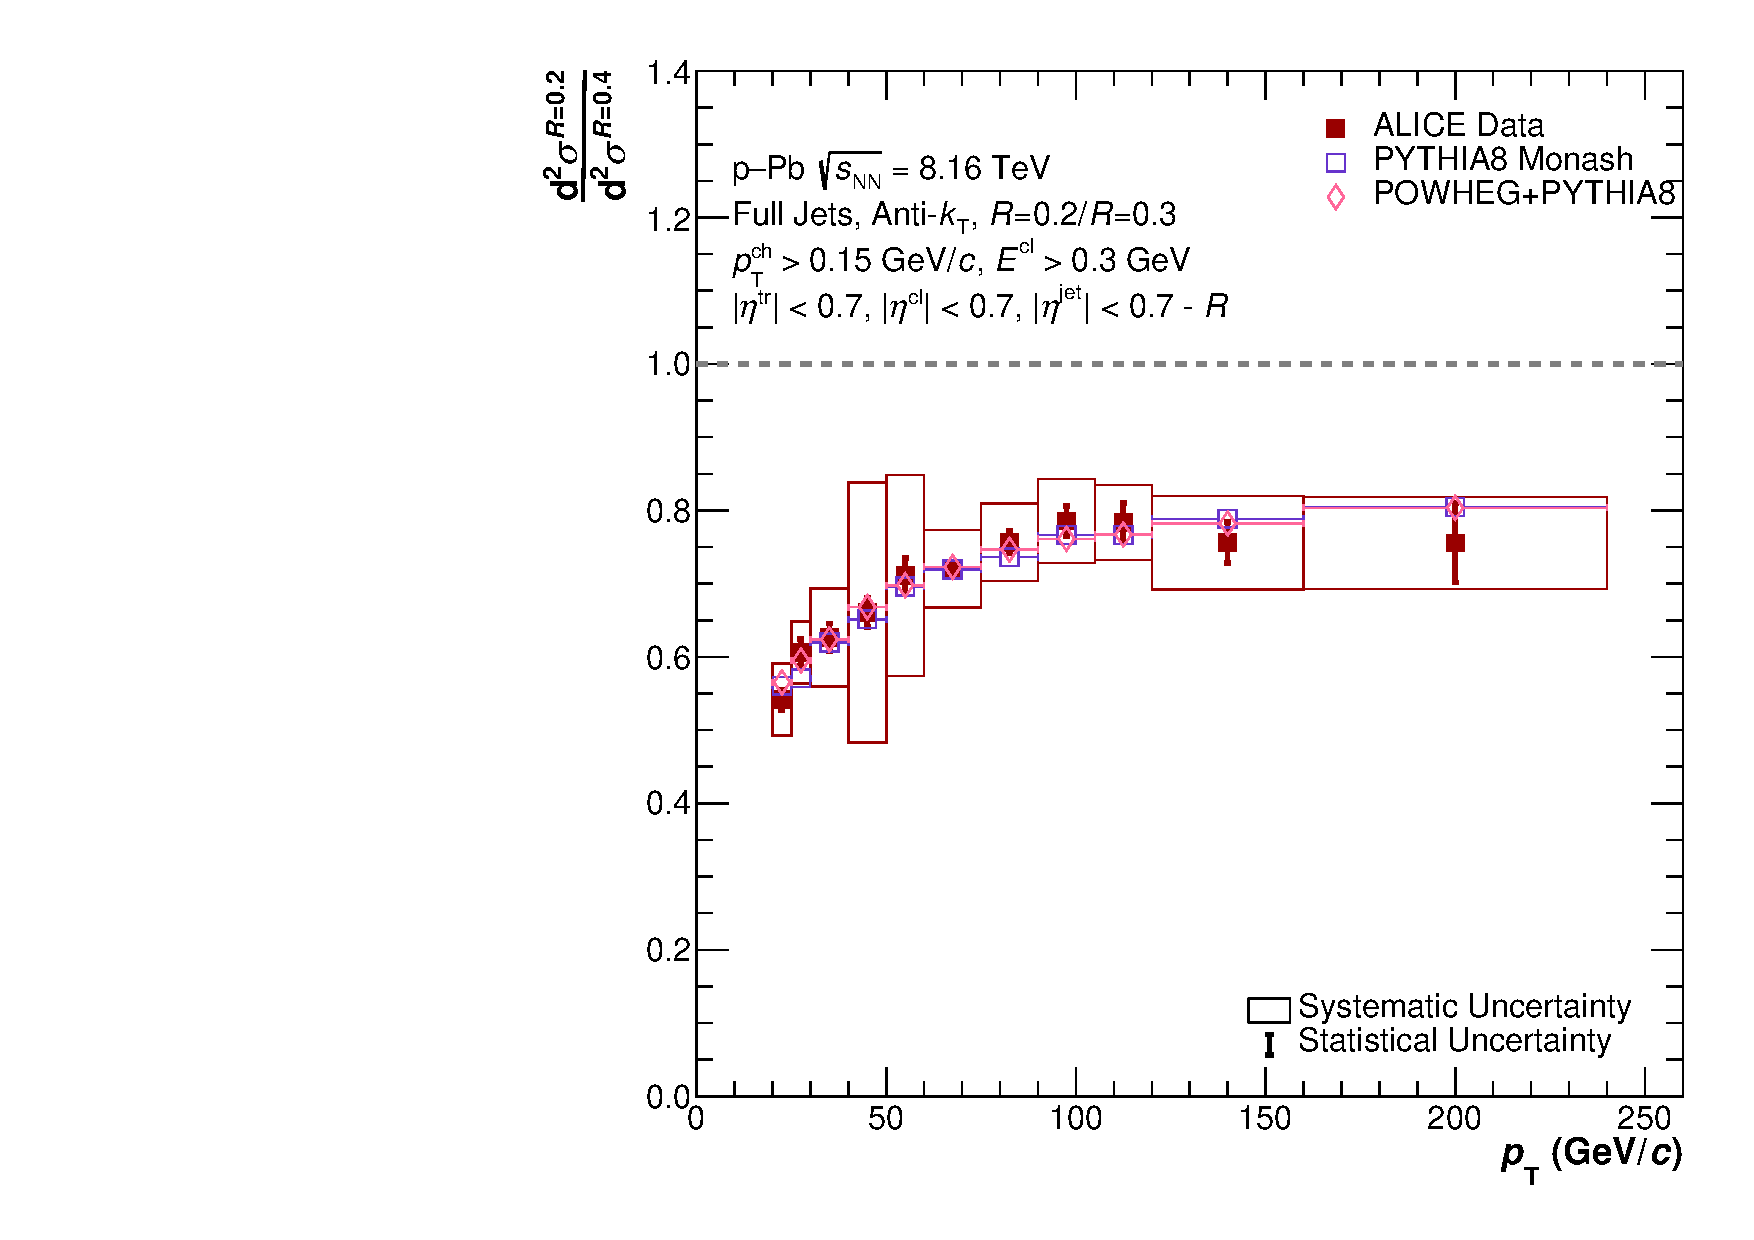
\includegraphics[width=7.5cm]{figures/pPbFigures/MCGen/MCComp_Ratio_R0302_nooutlier.pdf}
        \vfill\null
        \columnbreak
            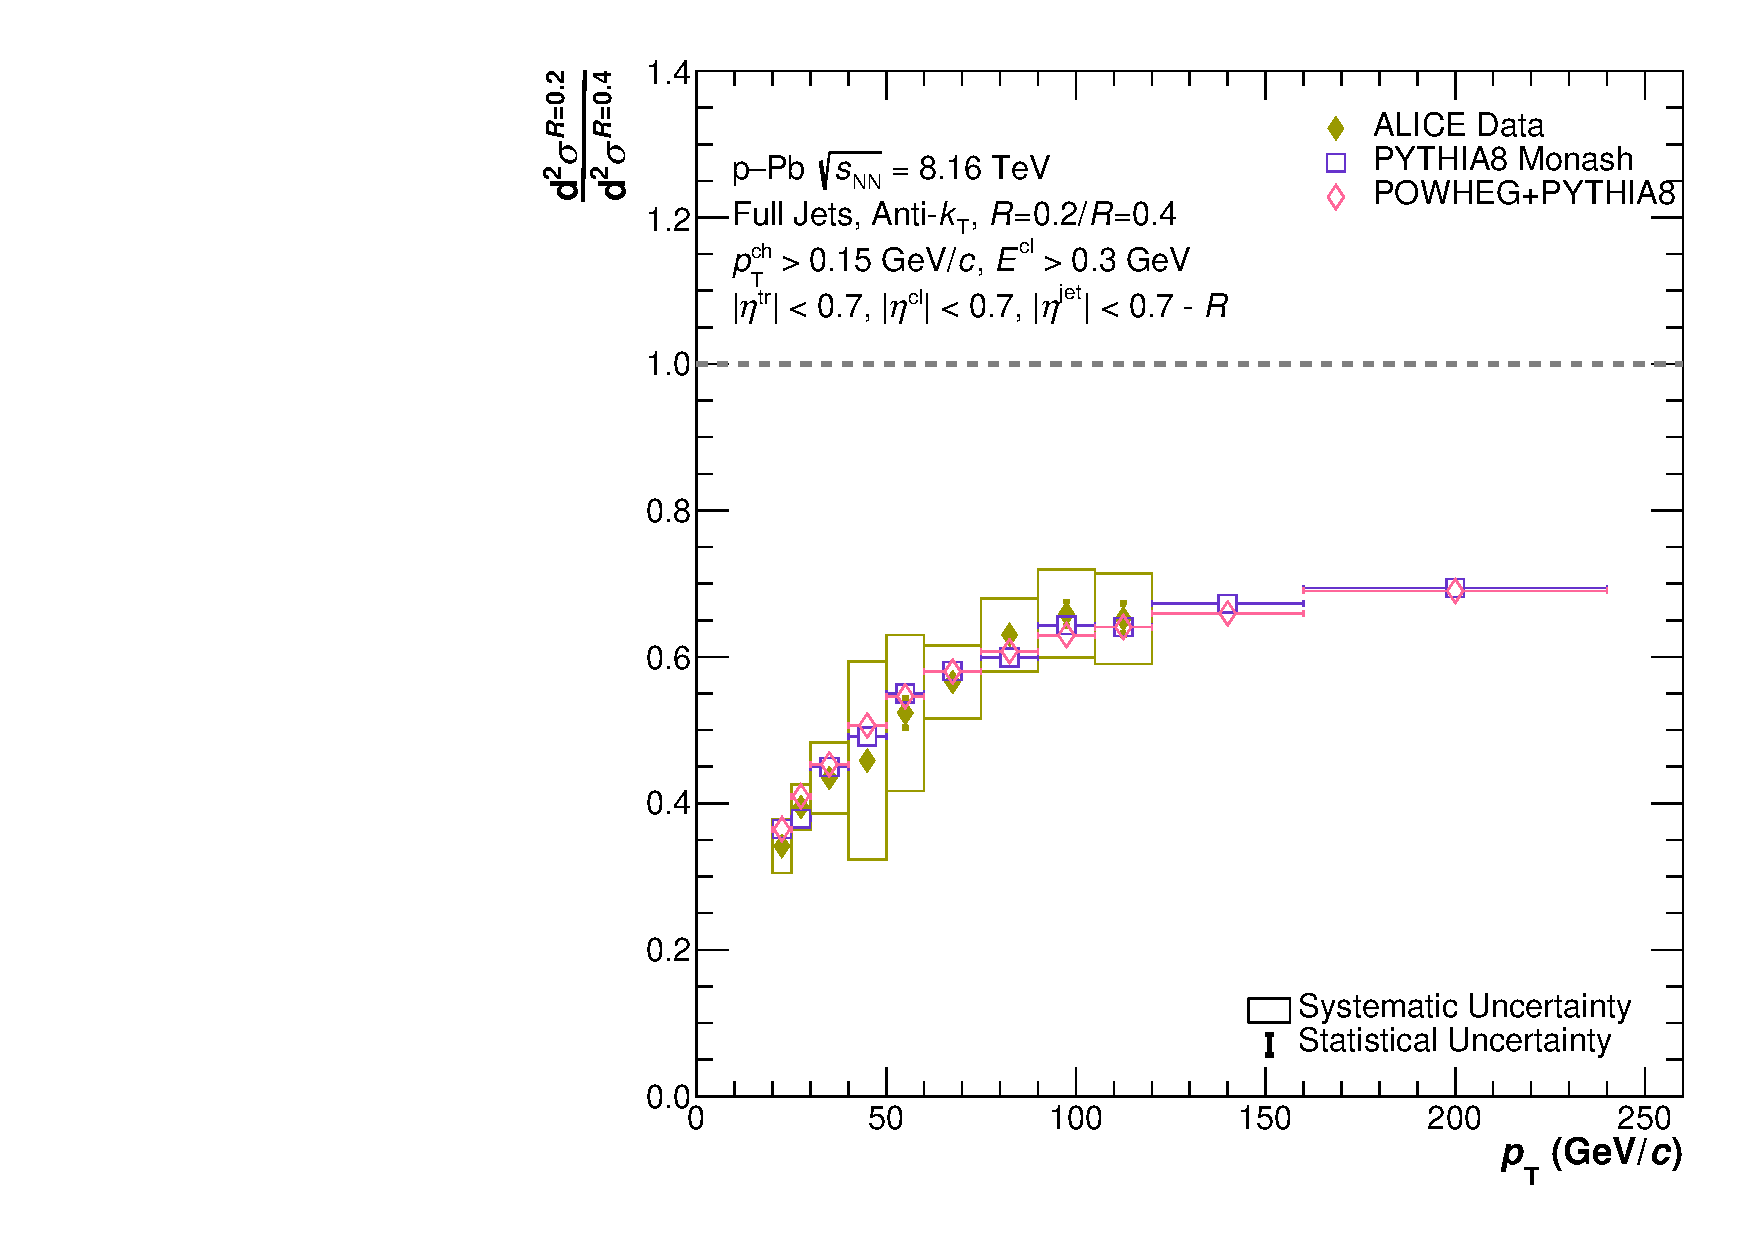
\includegraphics[width=7.5cm]{figures/pPbFigures/MCGen/MCComp_Ratio_R0402_nooutlier.pdf}
        \vfill\null
    \end{multicols}
    \caption{Comparison to PYTHIA8 Monash and POWHEG+PYTHIA8 for ratios of jet radii 0.2/0.3 and 0.2/0.4 in \pPb collisions.}
    \label{fig:MCGen_Ratio_pPb}
\end{figure}

\section{Collision Energy Dependence in \pp Collisions}
\label{sec:CollEnergyDep}

Figure~\ref{fig:specCompareR04} shows the jet cross-sections in \pp collisions at \s = 2.76, 5.02, 8, and 13 TeV for $R$ = 0.4. With increasing collision energy, it becomes more likely to create a high-momentum jet. This behavior is also seen in Figure~\ref{fig:sqrtSCompareR04}, which shows the collision energy dependence of the jet cross-section in \pp collisions for $R$ = 0.4 in various ranges of jet \pT. The spectra are fit with a power law in each \pT range. An increasing power law exponent is observed for increasing jet \pT.

\begin{figure}[hbt!]
    \centering
    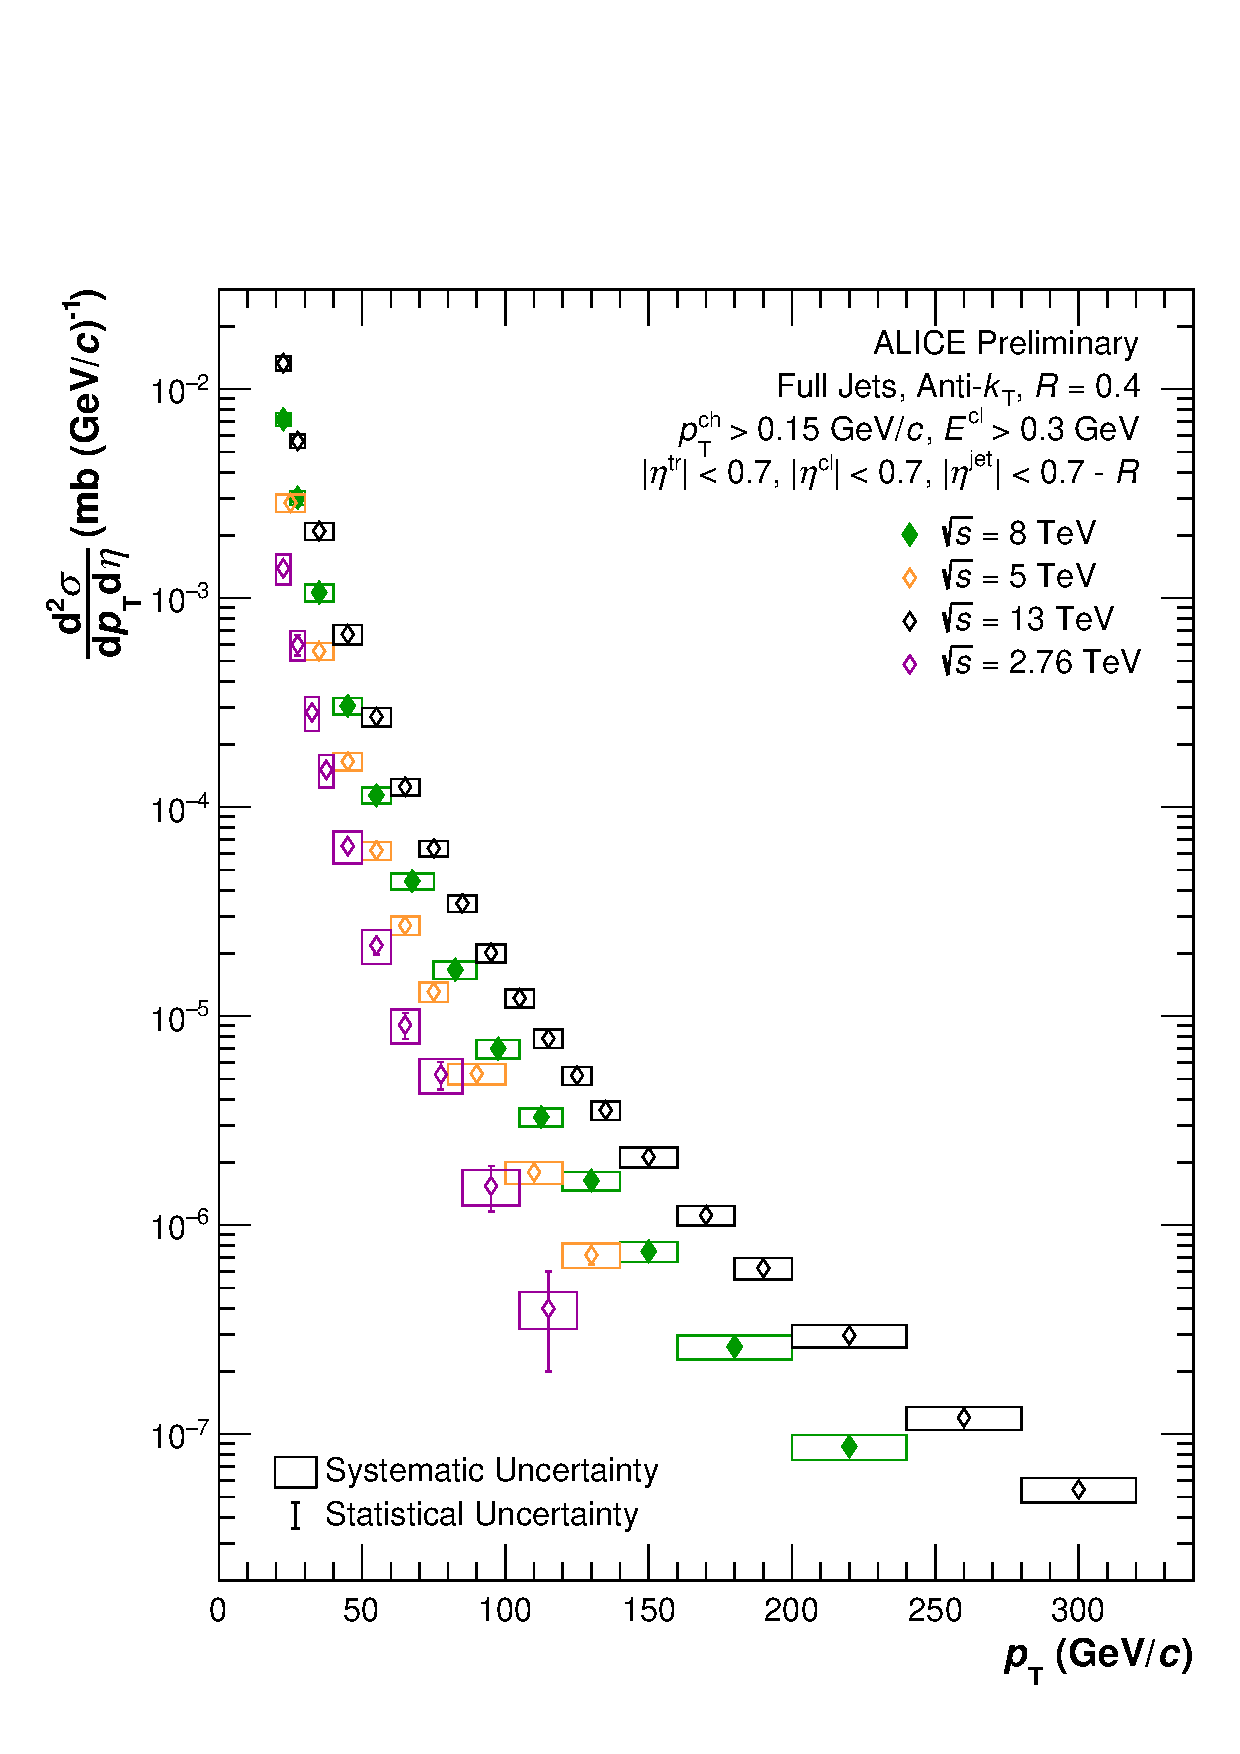
\includegraphics[width=\textwidth]{figures/EnergyComparisons/SpectrumComparison_R04.pdf}
    \caption{Jet cross-section measurements in \pp collisions at \s = 2.76, 5.02, 8, and 13 TeV for $R$ = 0.4.}
    \label{fig:specCompareR04}
\end{figure}

\begin{figure}[hbt!]
    \centering
    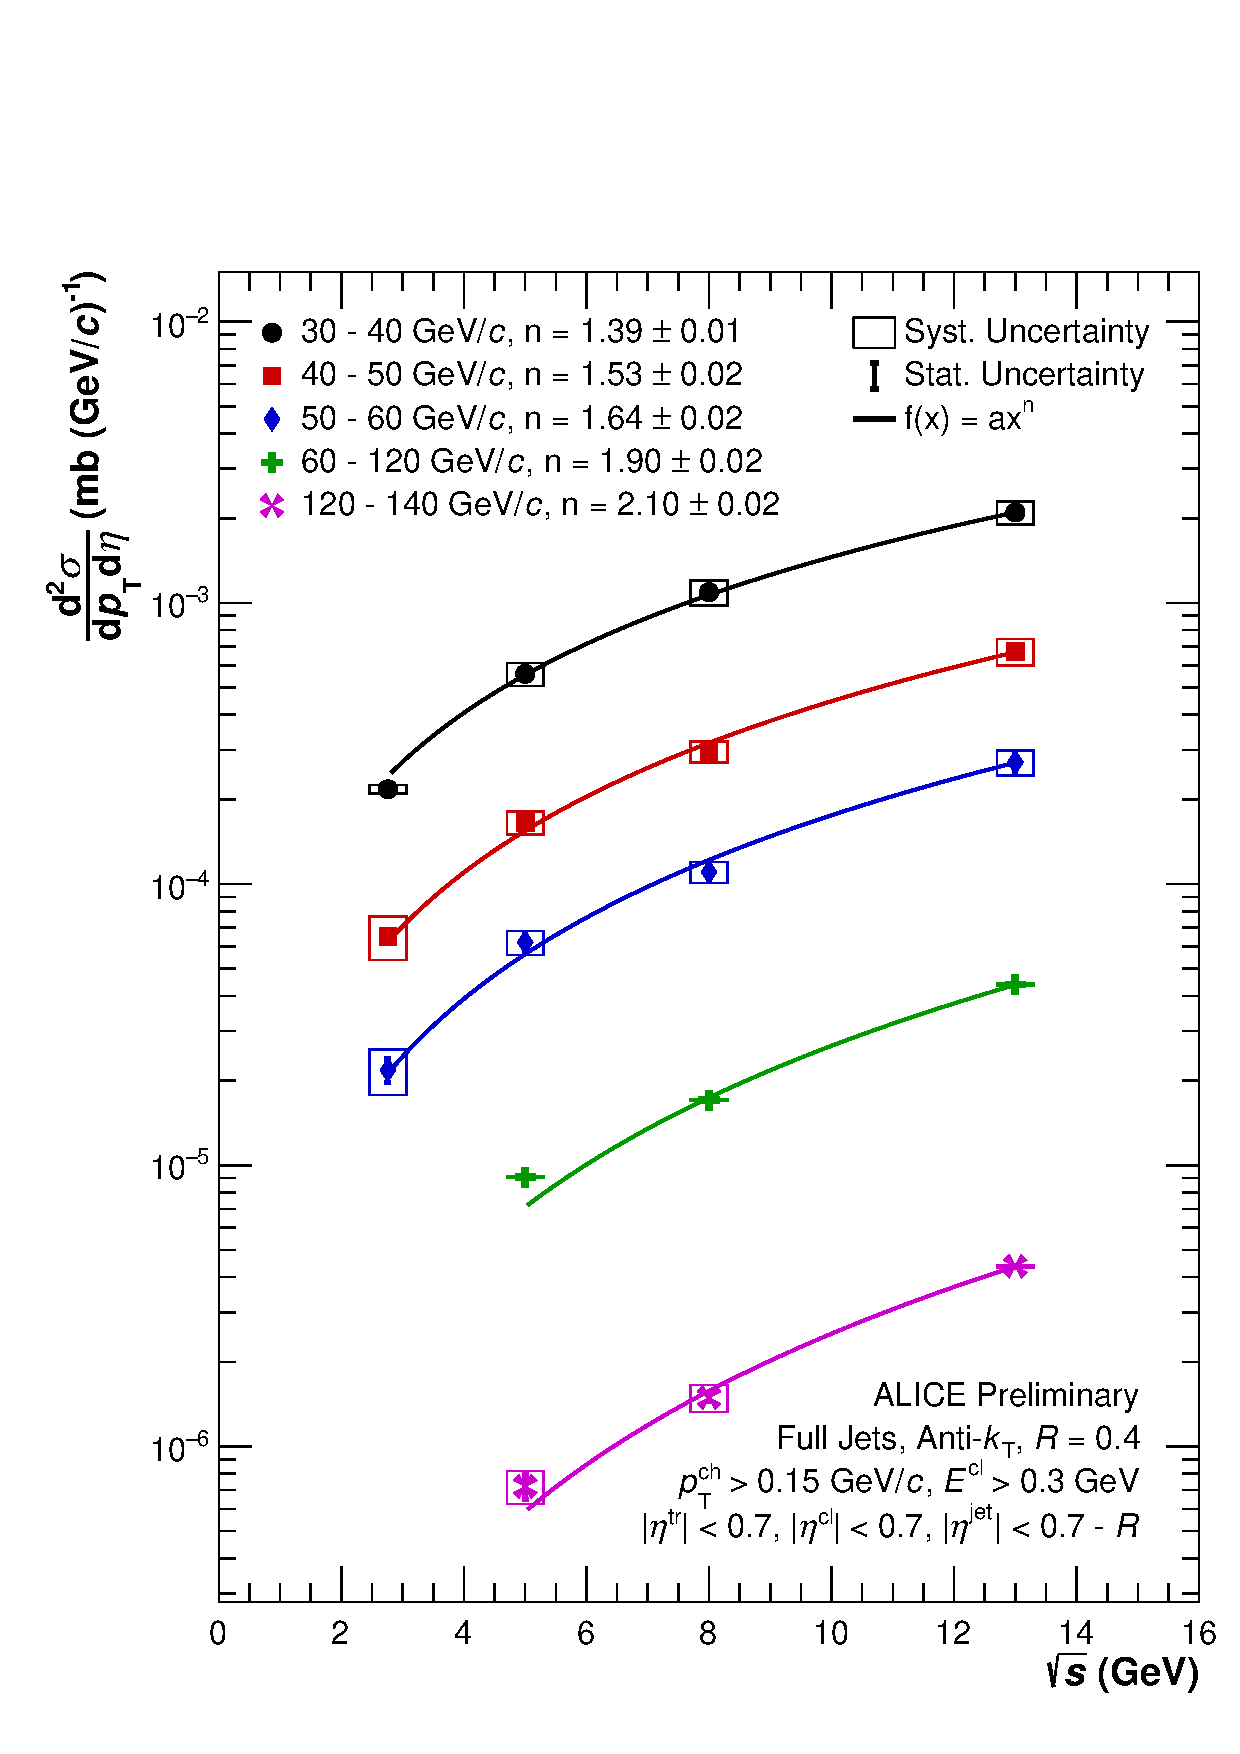
\includegraphics[width=\textwidth]{figures/EnergyComparisons/sqrtSComp_R04.pdf}
    \caption{Collision energy dependence of the jet cross-section in \pp collisions for $R$ = 0.4 in various ranges of jet \pT, fit with a power law in each \pT range.}
    \label{fig:sqrtSCompareR04}
\end{figure}

Figure~\ref{fig:ratioCompareR03} shows the ratios of the jet cross-sections for $R$ = 0.2/0.3 for \pp collisions at \s = 5.02, 8, and 13 TeV. The ratio is consistent between all collision energies within uncertainties, indicating that jet fragmentation pattern is similar between the different collision energies.

\begin{figure}[hbt!]
    \centering
    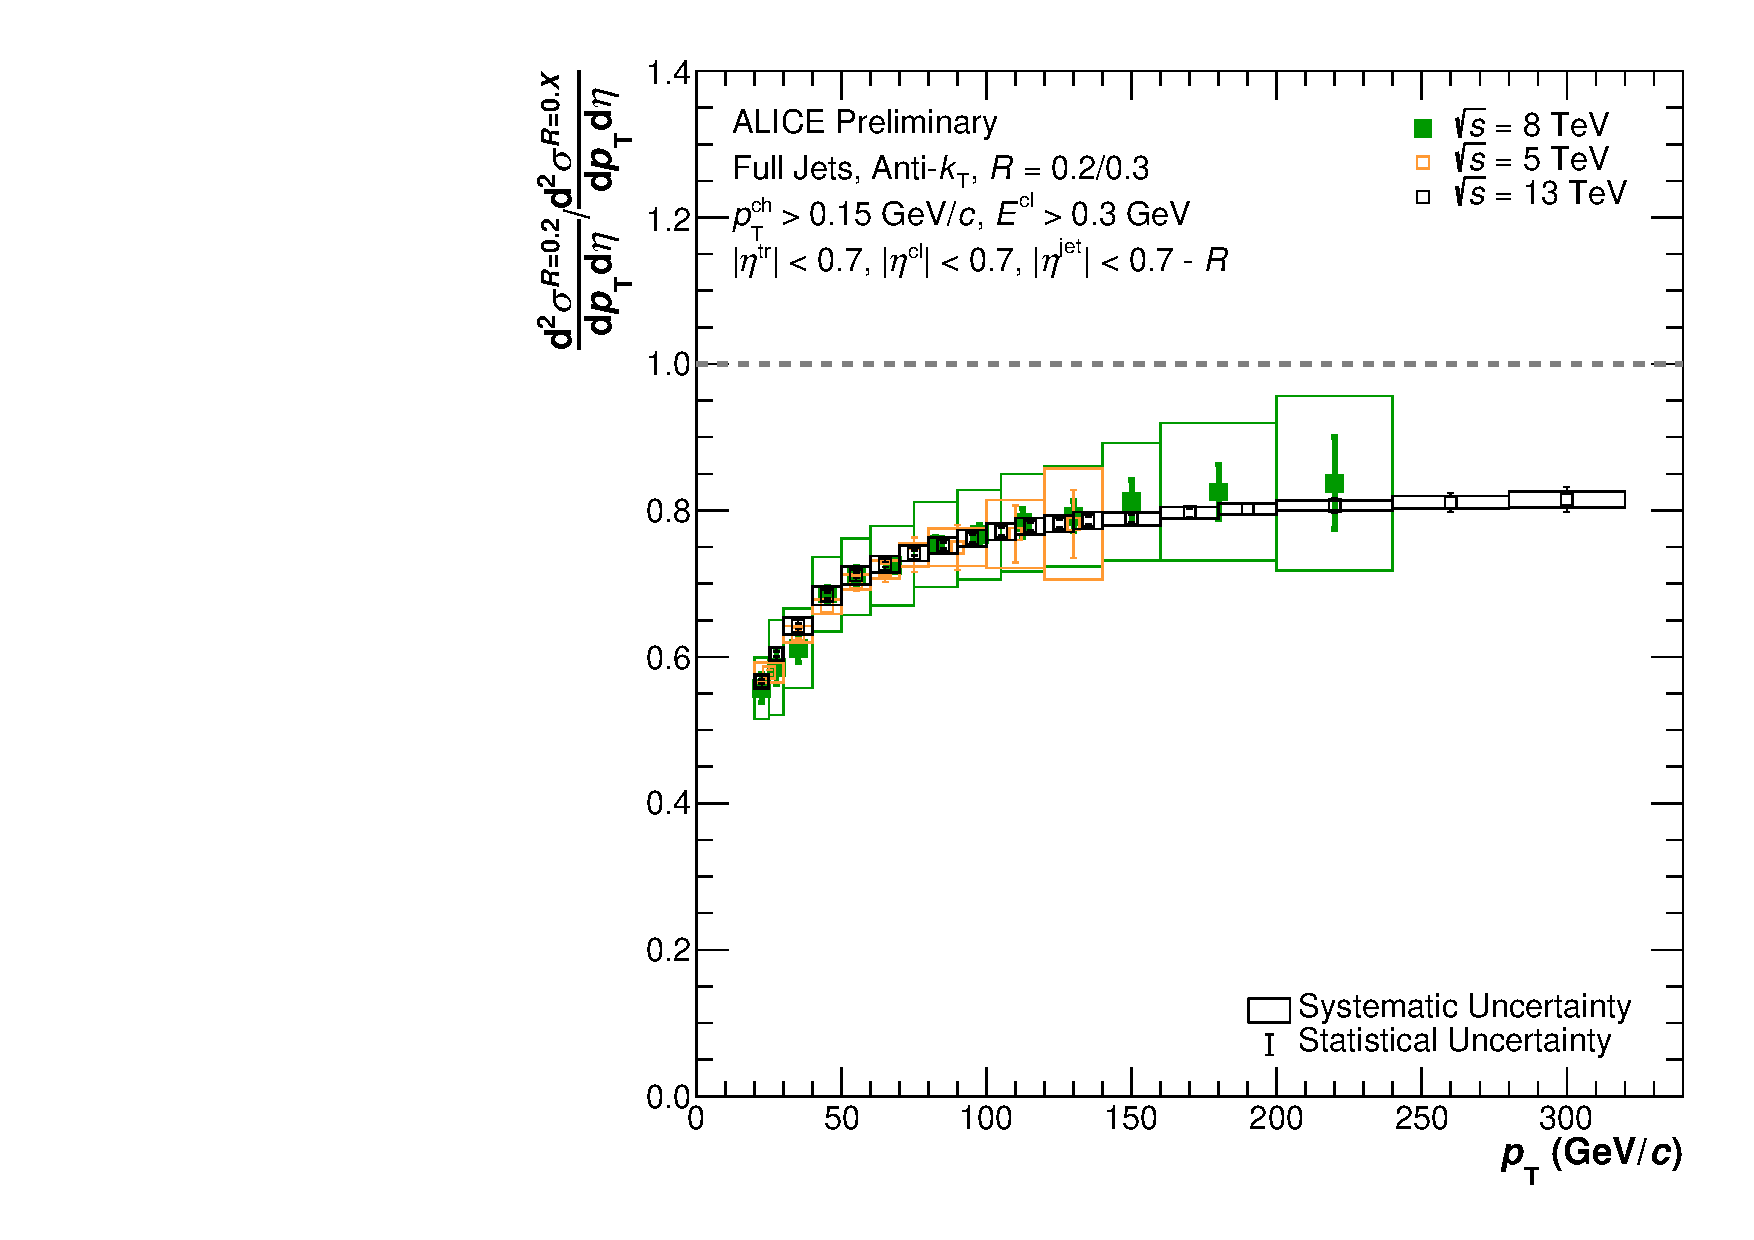
\includegraphics[width=\textwidth]{figures/EnergyComparisons/RatioComparison_R03.pdf}
    \caption{Ratio of jet cross-section measurements for $R$ = 0.2/0.3 in \pp collisions at \s = 5.02, 8, and 13 TeV.}
    \label{fig:ratioCompareR03}
\end{figure}

Collision energy dependence plots for the cross-section and ratios for the remaining jet resolution parameters can be found in Appendix~\ref{sec:appendixCollEnergyDep}.